\chapter{\ifproject%
      \ifenglish Project Structure and Methodology\else โครงสร้างและขั้นตอนการทำงาน\fi
  \else%
      \ifenglish Project Structure\else โครงสร้างของโครงงาน\fi
  \fi
 }

ในบทนี้จะกล่าวถึงหลักการ, การนำทฤษฎีที่เกี่ยวข้องมาประยุกต์ใช้ และการออกแบบของระบบ

\makeatletter

% \renewcommand\section{\@startsection {section}{1}{\z@}%
%                                    {13.5ex \@plus -1ex \@minus -.2ex}%
%                                    {2.3ex \@plus.2ex}%
%                                    {\normalfont\large\bfseries}}

\makeatother
%\vspace{2ex}
% \titleformat{\section}{\normalfont\bfseries}{\thesection}{1em}{}
% \titlespacing*{\section}{0pt}{10ex}{0pt}

\section{การจัดเก็บข้อมูล}
โดยข้อมูลราคาหุ้นทุกตัวจะมีแหล่งที่มาจาก AlphaVantage โดยจะให้ข้อมูลย้อนหลังไป 2 ปี และใช้อัพเดท
ข้อมูลแบบทุกๆ 30 นาที และในส่วนของราคา Crypto-Currency จะมีแหล่งที่มาจาก Binance ทั้งหมดซึ่งมีการอัพเดททุกๆ 30 นาทีเช่นกัน
เราใช้ MongoDB เป็น Database สำหรับจัดเก็บข้อมูลตลาดหุ้น

ในตอนเริ่มตันนั้นเราดึงข้อมูลที่ต้องการมาจาก AlphaVantage API ซึ่งได้มาเป็นข้อมูลตลาดหุ้นย้อนหลัง 2 ปีโดย
และเก็บข้อมูลลง MongoDB โดยมีการแปลงข้อมูลให้เป็นในรูปแบบข้อมูลตลาดของเราซึ่งก็จะประกอบด้วย
\begin{enumerate}
    \item ticker: ชื่อของหุ้นที่ทำการซื้อขาย เช่น AAPL/USD, TSLA/USD, ETH/USDT
    \item open: เป็นราคาซื้อขายแรกที่เกิดขึ้นใน ช่วงเวลานั้นๆ
    \item close: เป็นราคาสุดท้ายที่เกิดขึ้นจากการซื้อขายสิ้นสุด ของช่วงเวลานั้นๆ
    \item high: การเคลื่อนไหวของราคาหุ้น ณ ระดับราคาสูงสุดในช่วงเวลานั้นๆ
    \item low: การเคลื่อนไหวของราคาหุ้น ณ ระดับราคาต่ำสุดในช่วงเวลานั้นๆ
    \item volume: ปริมาณการซื้อขายในช่วงเวลานั้นๆ
\end{enumerate}
จากนั้นในการอัพเดตข้อมูลทุกๆ 30 นาที เราจะใช้ Amazon EventBridge Scheduler ที่จะไปเรียกใช้ AWS Lambda ที่เราสร้างขึ้นมาโดยใน Lambda จะดึงข้อมูลจาก
AlphaVantage มาอัพเดต ในส่วนของ Crypto-Currency ก็จะใช้ระบบแบบเดียวกันแต่จะใช้ Binance API ทั้งในการดึงข้อมูลครั้งแรกและการอัพเดตแทน

\begin{figure}[ht]
    \centering
    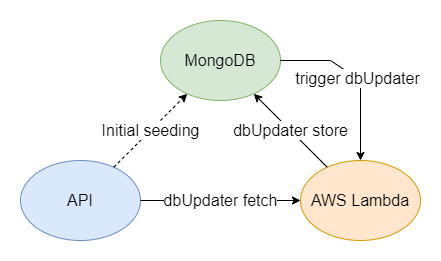
\includegraphics[scale=0.6]{images/db.png}
    \caption{โครงสร้างของการจัดเก็บข้อมูล โดนเส้นประคือทำครั้งเดียวในตอนแรกเริ่ม และเส้นทึบจะทำในทุกๆ ชม. โดยเป็นการเรียกใช้โปรแกรม dBUpdater ใน AWS Lambda}
    \label{fig:7}
\end{figure}
\FloatBarrier

\section{การสร้างตัวชี้วัดทางเทคนิคด้วย Fuzzy Logic}
เราจะใช้ Mamdani Fuzzy Inference System กับตัวแปรทางภาษาและ Fuzzy Rule ที่จะกล่าวด้านล่างนี้ในการคำนวณค่าสัญญาณของเรามา โดย defuzzification method จะใช้แบบ
centroid

\subsection{ตัวแปรทางภาษา (Linguistic Variable)}
สำหรับตัวชี้วัดทางเทคนิคแต่ละตัวที่เรามีให้ได้แก่ Relative Index Strength (RSI), Bollinger Band (BB), Moving Average Convergence/Divergence
(MACD), Average Directional Index (ADX), Aroon oscillator (AROON), On-Balance Volume (OBV), Stochastic Oscillator,
Accumulation/Distribution Indicator (A/D) ซึ่งผู้ใช้สามารถใช้ระบบของเราผ่านเว็บแอปพลิเคชัน ในการสร้างตัวแปรทางภาษาจากแต่ละตัวชี้วัดทางเทคนิค
และก็สามารถสร้างตัวแปรทางภาษาสำหรับสัญญาที่จะออกมายกตัวอย่างเช่น ทำป็นสัญญาณ long (ควรเข้า position long) และสัญญาณ short (ควรเข้า position short)
ซึ่งจะคิดมาจากตัวแปรทางภาษาของตัวชี้วัดทางเทคนิคที่กล่าวถึงด้านบน ยกตัวอย่างตัวแปรทางภาษาที่เราอาจจะใช้บนรูปที่ \ref{fig:8}
\begin{figure}[ht]
    \centering
    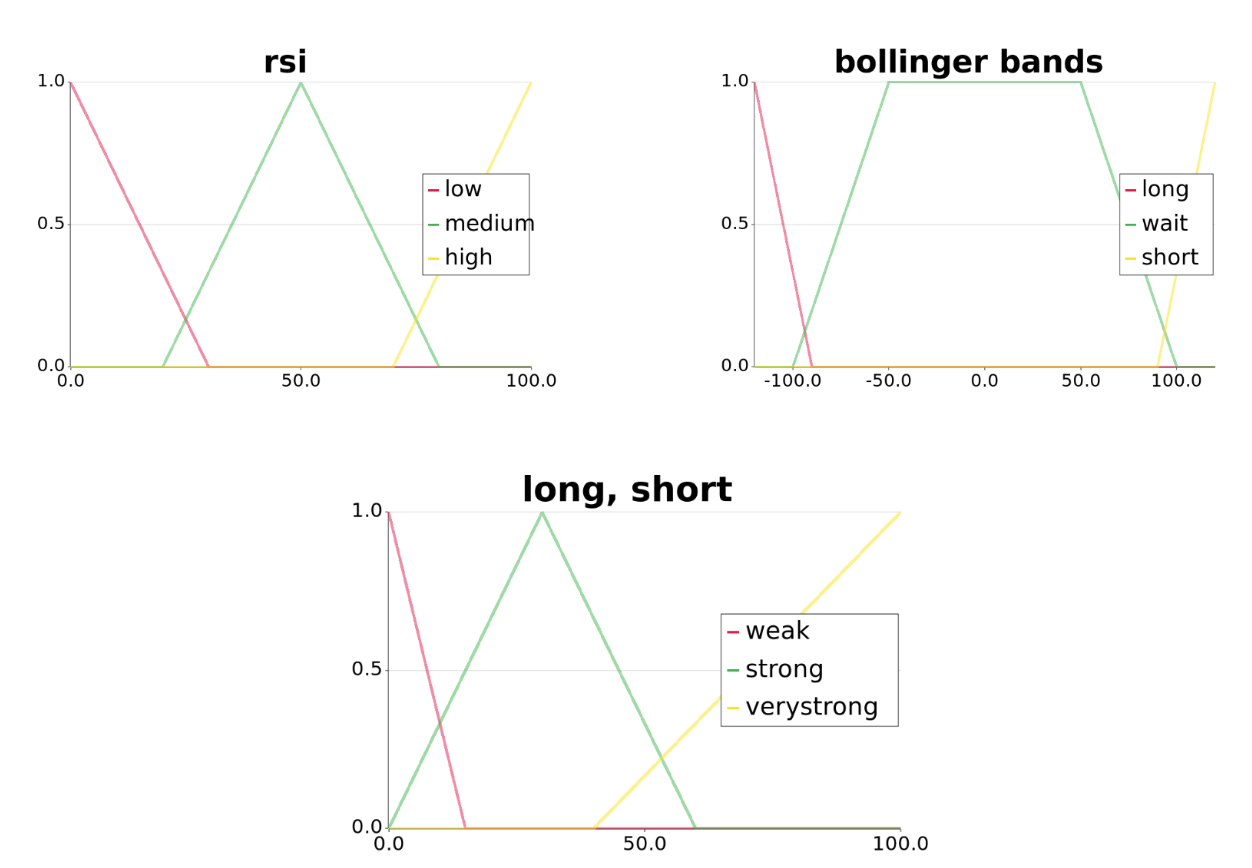
\includegraphics[width=\textwidth]{images/linguistic.png}
    \caption{ตัวแปรทางภาษาสำหรับ RSI, Bollinger Band, long, short}
    \label{fig:8}
\end{figure}

\subsection{Fuzzy Rules}
เราจะใช้การตีความทั่วๆไปของแต่ละตัวชี้วัดมาสร้าง Fuzzy Rule เริ่มต้น ยกตัวอย่างเช่นถ้าเราใช้แค่ RSI และ Bollinger Band ในการสร้าง long และ short เราจะมี fuzzy rule
เหมื่อนในตารางที่ \ref{table:1} โดยในระบบของเราจริงๆ เราจะใช้ตัวแปรทางภาษาที่เรากล่าวในหัวข้อก่อนหน้ามาทั้งหมดสร้าง Fuzzy Rule ในการสร้างสัญญาณ long และ short และเรา
จะออกแบบระบบให้ผู้ใช้สามารถปรับแต่งกฏตรงนี้ได้ในทั้ง website

\begin{table}[htp]
    \centering
    \begin{tabular}{c c c c}
        \toprule
        {RSI}  & {Bollinger Bands} & {LONG}     & {SHORT}    \\
        \midrule
        HIGH   & LONG              & WEAK       & WEAK       \\
        HIGH   & WAIT              & WEAK       & STRONG     \\
        HIGH   & SHORT             & WEAK       & VERYSTRONG \\
        MEDIUM & LONG              & WEAK       & STRONG     \\
        MEDIUM & WAIT              & WEAK       & WEAK       \\
        MEDIUM & SHORT             & STRONG     & WEAK       \\
        LOW    & LONG              & VERYSTRONG & WEAK       \\
        LOW    & WAIT              & STRONG     & WEAK       \\
        LOW    & SHORT             & WEAK       & WEAK       \\
        \bottomrule
    \end{tabular}
    \caption{ตัวอย่างของ Fuzzy Rules ที่ใช้แค่ RSI และ Bollinger Band เพื่อสร้าง long และ short.}
    \label{table:1}
\end{table}
\FloatBarrier

\section{การปรับแต่ง Fuzzy Logic ด้วย PSO}
เป้าหมายของเราในการปรับแต่ง Fuzzy Logic ที่ใช้สำหรับการสร้างตัวชี้วัดทางเทคนิคใหม่ของเรานั้น ก็คือการปรับแต่งตัวแปรทางภาษาต่างๆ ที่มีอยู่ fuzzy rules เพื่อให้
ตัวชี้วัดทางเทคนิคของเรานั้นสามารถสร้างกำไรได้มากที่สุดใน\emph{วิธีการเทรดที่เราใช้ปรับแต่ง} โดยเราจะใช้ PSO (Particle Swarm Optimization) ในการปรับพารามิเตอร์ที่ใช้
สร้างตัวแปรทางภาษาแต่ละอัน โดยพารามิเตอร์ในการสร้าง fuzzy set นั้นจะแตกต่างกันไปตามรูปแบบของ fuzzy set
เช่นถ้าเป็นแบบสามเหลี่ยมก็จะมีพารามิเตอร์ดังที่เห็นในรูปที่ \ref{fig:9} โดยผู้ใช้งานจะสามารถใช่ PSO ในการปรับแต่งตัวแปรทางภาษาได้เองผ่าน website ที่เราจัดทำขึ้นมา

\begin{figure}[ht]
    \centering
    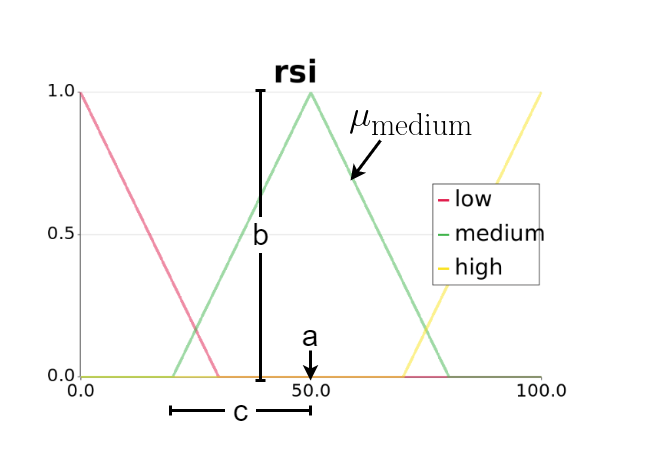
\includegraphics[width=0.8\textwidth]{images/linguisticv.png}
    \caption{ตัวแปรทางภาษาและตัวแปรที่เราต้องการจะปรับแต่ง $\mu_{\text{medium}} = b (1 - \frac{ |x-a| }{s})$ (ในที่นี้คือเราจะปรับแต่งค่าของ $a, b, s$)}
    \label{fig:9}
\end{figure}

\subsection{กลยุทธ์ที่เราใช้ปรับแต่ง}
โดยในการปรับแต่ง Fuzzy Logic ของเรานั้นอันดับแรกเลยเราต้องเลือกกลยุทธ์การเทรดที่เราต้องการปรับแต่ง ให้มีผลต่อตัวชี้วัดทางเทคนิค ยกตัวอย่างกลยุทธ์การเทรด
เช่น มีเงินต้น 2000 บาท ถ้า buySignal มากกว่า 50 ให้เข้าซื้อด้วย 100 บาท ด้วย stop-loss ที่ 10\% และ take profit ที่ 20\%
\subsection{Backtesting}
Backtesting คือการนำกลยุทธ์การเทรดที่เราเลือก ไปใช้กับข้อมูลในอดีตในกรอบเวลาที่ผ่านๆ มาเพื่อทดสอบว่ากลยุทธ์นั้นไปใช้ในตลาดจริงๆ ในอดีตแล้วได้ผลดีแค่ไหน
โดยเราสามารถเลือกกรอบเวลาที่ตลาดมีลักษณะคล้ายๆ กับในปัจจุบัน แล้วลองปรับเปลี่ยนและทดสอบกลยุธ์การเทรดนั้นๆ ได้เพื่อให้ได้ผลลัพธ์ที่เราต้องการ

โดยเราจะทำการ backtest ด้วยกลยุทธ์การเทรดที่เราเลือกมา แล้วเก็บข้อมูลการเทรดที่เกิดขึ้นทั้งหมดโดยแต่ละการเทรดจะมีข้อมูลดังนี้
\begin{itemize}
    \item เวลาที่เข้า position
    \item เวลาที่ออก position
    \item ราคาที่เข้าซื้อ
    \item ราคาที่ขาย
    \item จำนวนเงินที่จ่ายไป
    \item กำไรขาดทุนที่ได้ ($\text{realizedPnl}$)
\end{itemize}

\subsection{Objective Function}
เราจะใช้ Objective Function ที่คำนวณมาดังนี้ 
$$ f = 
\begin{cases}
    \infty & |\text{trades}| = 0 \\
    -1 \times ((\text{np} - \text{np}_r) + (\text{mdd}_r - \text{mdd})) & \text{otherwise} \\ 
\end{cases}
$$ 
โดยที่
\begin{itemize}
    \item {$\text{np} = \frac{\sum_{i=0}^{n} p_i(\text{realizedPnl})}{\text{startMoney}}$
          คือ Net Profit ที่มีค่าอยู่ในช่วง $[0, \infty)$ ซึ่งได้จากการเทรดทั้งหมดโดยคำนวนจากข้อมูลการเทรดที่เราได้จากการทำ backtest โดย $n$ คือจำนวนข้อมูลทั้งหมด
          และ $p_i(\text{realizedPnl})$ คือข้อมูลตัวที่ $i$ โดยเอาค่า $\text{realizedPnl}$ มา
          }
    \item {$\text{mdd}$ (Maximum Drawdown ตัวอย่างในรูปที่ \ref{fig:10}) มีค่าอยู่ในช่วง $[0, 1]$ โดยเราสามารถคิดค่านี้โดยให้
          $$
              g(x) = \sum_{i = 0}^{x}p_i(\text{realizedPnl})
          $$
          \begin{equation}
              \text{mdd}' = \max_{r \in (0, n)} \left[ \max_{t \in (0, r)} g(t) - g(r) \right]
          \end{equation}
          แล้วให้เราจำค่า $y = g(t)$ ที่ทำให้ได้
          $\text{mdd}'$ เยอะที่สุดไว้ แล้วจะได้ว่า $\text{mdd} = \frac{\text{mdd}'}{y}$
          }
    \item {$|\text{trades}|$ คือจำนวนของการซื้อขายที่เกิดขึ้นในการ backtest}
    \item {$\text{np}_r$ และ  $\text{mdd}_r$ คือค่า Net Profit และ Maximum Drawdown ที่เราได้จากการ backtest โดยใข้ตัวแปรทางภาษาตั้งต้นก่อนที่จะทำการ
          ฝึกสอนด้วย PSO โดยเราจะใช้ค่านี้เป็นตัวอ้างอิงไว้เปรียนเทียบกับผลลัพธ์ของการปรับแต่งตัวแปรทางภาษาเพื่อให้เราได้ผลที่ไม่แย่ไปกว่าตัวแปรทางภาษาแบบเดิม
          }
\end{itemize}
ในส่วนของ hyper parameters ต่างๆ ที่เราต้องตั้งให้ PSO algorithm เช่น จำนวน particles, การคำนวณ velocity เป็นต้น จะเปลี่ยนไปตามแต่ละครั้งของการปรับแต่ง
โดยเราจะทดลองหลายๆ แบบเพื่อให้ได้ตัวชี้วัดที่มีประสิทธิภาพดีที่สุด

\begin{figure}[ht]
    \centering
    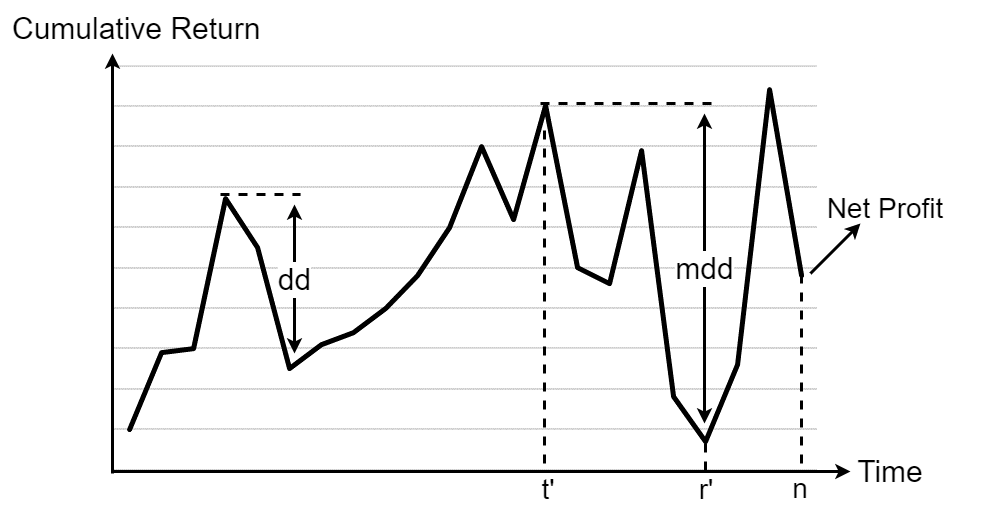
\includegraphics[width=0.8\textwidth]{images/mdd.png}
    \caption{ตัวอย่างของ Net Profit และ Maximum Drawdown}
    \label{fig:10}
\end{figure}

\section{การจัดการเงินทุน}
เราจะใช้ optimal-f (\cite{Vince}) ที่ถูกดัดแปลงตามที่ \cite{Rodrigo} ได้ทำไว้ในส่วนของการจัดการเงินทุน ซึ่งจะบอกเราว่าควรลงทุุนโดยใช้เงินเท่าไหร่ เพื่อให้เงินกำไรเติบโตแบบ
exponential โดยจะคิดมาจากผลลัพธ์ของการเทรดก่อนหน้า ถ้าเราเทรดสำเร็จเยอะก็จะเพิ่มเงินที่จะลงทุน ถ้าเทรดพลาดเยอะก็จะลดเงินที่จะลงทุน

อันดับแรกให้เราหาค่า $f$ ที่ทำให้ terminal wealth relative ($\text{TWR}$) ในสมการ \ref{eq:twr} มีค่ามากที่สุด
\begin{equation}
    \text{TWR}(f) = \Pi_{i=1}^{n} \text{HPR}_i(f)
    \label{eq:twr}
\end{equation}
\begin{equation}
    \text{HPR}_i(f) = 1 + \frac{f \cdot p_i(\text{realizedPnl})}{\text{riskFactor}}
\end{equation}
โดยที่ $\text{HPR}$ คือ holding perioid return หรือก็คืออัตราส่วนกำไรขาดทุนของแต่ละ position
,$n$ คือจำนวน position ทั้งหมด, $p_i(\text{realizedPnl})$ คือกำไรขาดทุนของ position ที่ $i$,
และ $\text{riskFactor}$ คือค่าสัมบูรณ์ของ $p_i(\text{realizedPnl})$ ที่แย่ที่สุด

แต่ในปรกติแล้วค่า $f$ ที่เราได้มานั้นจะมีความเสี่ยงมากเกินไปเราก็จะใช้เป็น liquid-F ที่เป็น 10\% ของ $f$ เป็น $\text{liquid}_f = 0.1f$
\begin{equation}
    \text{size} = \text{liquid}_f + \frac{(\text{output} - \text{threshold}) \cdot (f - \text{liquid}_f)}{\text{output}_{\text{max}} - \text{threshold}}
\end{equation}
โดย $\text{output}$ คือค่าจากสัญญาน long หรือ short ของเรา, $\text{threshold}$ คือค่าที่ $\text{output}$ ที่ต่ำที่สุดที่เราจะเข้า position, และ
$\text{output}_{\text{max}}$ คือค่าที่มากที่สุดที่เป็นไปได้ของ $\text{output}$ จากนั้นเราก็นำ $\text{size}$ ไปคำนวณจำนวนที่จะลงทุนด้วยสมการ \ref{eq:shares}
\begin{equation}
    \text{amount} = \frac{C \cdot \text{size}}{\text{price}}
    \label{eq:shares}
\end{equation}
โดย $C$ คือจำนวนเงินที่เราทำไปลงทุนได้ และ $\text{price}$ คือราคาของสินทรัพย์ที่เราจะลงทุน แล้วถ้าเรามี $C$ ไม่พอให้เราลงทุนมากที่สุดเท่าที่จะทำได้

\section{แผนภาพกระแสข้อมูลโดยรวมของระบบ (Data Flow Diagram)}
แผนภาพแสดงกระแสข้อมูลโดยเริ่มตั้งแต่การดึงข้อมูลตลาดจาก API มาเก็บที่ Database ซึ่งข้อมูลในนั้นจะถูกนำมาใช้งานคำนวณตัวชี้วัดทางเทคนิค, ประมวลผลและปรับตั้งระบบฟัซซี จนกระทั่งได้สัญญาณจากระบบฟัซซีไปแสดงบนเว็บแอปพลิเคชันให้กับผู้ใช้งาน
\begin{figure}[ht]
    \centering
    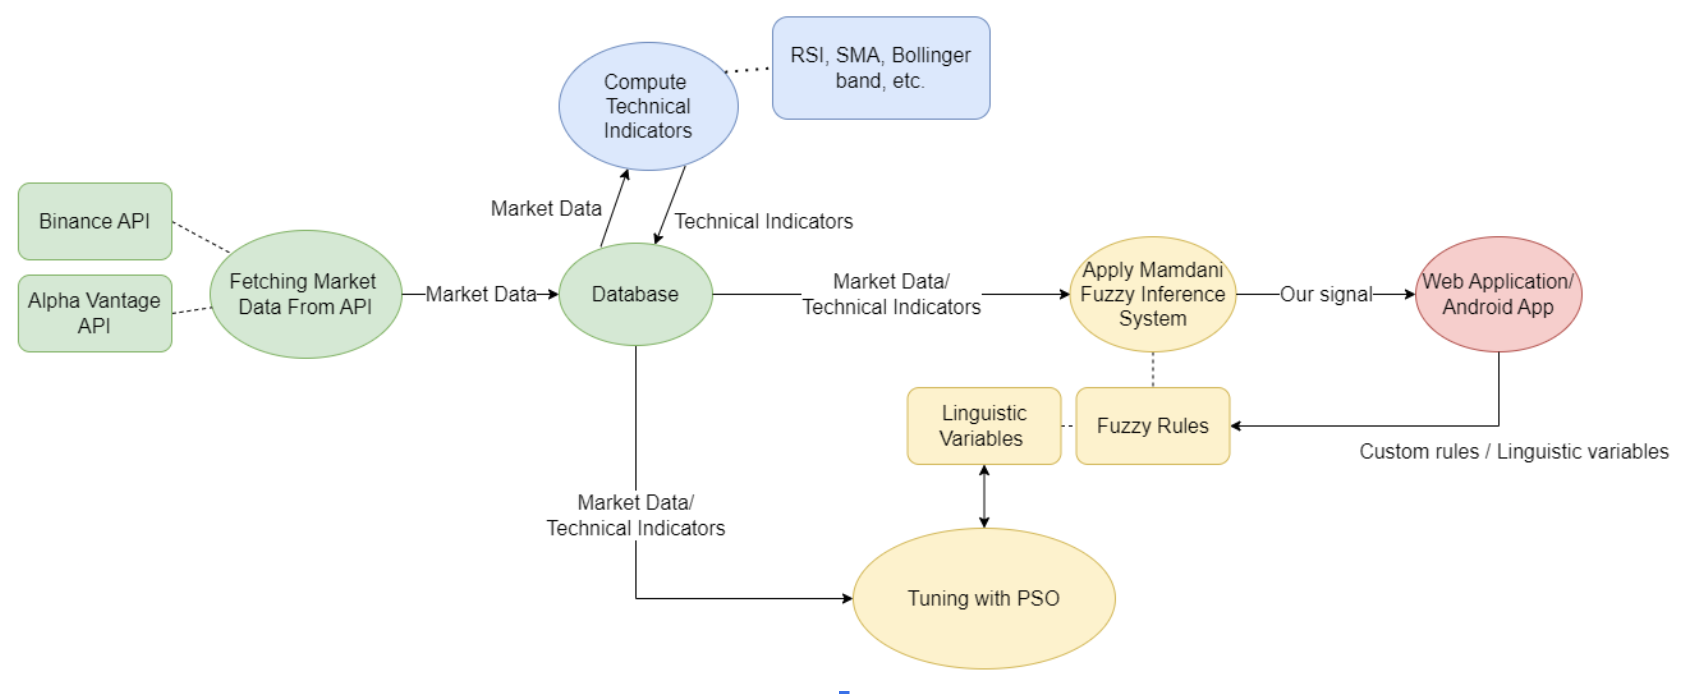
\includegraphics[scale=0.3]{images/overview.png}
    \caption{แผนภาพกระแสข้อมูล}
    \label{fig:11}
\end{figure}

\section{เว็บแอปพลิเคชัน}
เว็บแอปพลิเคชันสามารถรองรับการทำงานของผู้ใช้งานทั้งบนคอมพิวเตอร์และโทรศัพท์มือถือ \\
จุดประสงค์ของเว็บแอปพลิเคชันคือเป็นส่วนติดต่อให้กับผู้ใช้งานที่ต้องการเข้ามาใช้ระบบของเราโดยมีส่วนที่ต้องรองรับหลักดังนี้
\begin{itemize}
    \item ผู้ใช้งานสามารถดูกราฟ OHLC ของสินทรัพย์ในแต่ละ Interval
    \item ผู้ใช้งานสามารถเพิ่มเครื่องมือตัวชี้วัดเบื้องต้นที่ต้องการอย่างเช่น RSI, MACD, และตัวอื่นๆที่ระบบของเรามีให้
    \item ผู้ใช้งานสามารถสร้าง Preset และปรับแต่งระบบ Fuzzy logic (ปรับกฏ และตัวแปรทางภาษา)
    \item ผู้ใช้งานสามารถดูผลลัพธ์ที่ได้จาก Preset ระบบ Fuzzy logic
    \item ผู้ใช้งานสามารถทำการทดสอบกลยุทธ์ย้อนหลัง Backtesting บน Preset Fuzzy logic และดูผลลัพธ์การทดสอบ
    \item ผู้ใช้งานสามารถทำปรับจูนตัวแปรทางภาษาของ Preset Fuzzy logic ด้วย PSO และดูผลลัพธ์การปรับจูน
\end{itemize}
ทำการออกแบบ UI/UX ของเว็บแอปพลิเคชัน Figma
โดยในการพัฒนาเว็บแอปพลิเคชันส่วนหลักใช้ UI Framework อย่าง SvelteKit และภาษา TypeScript

\subsection{เว็บเซิร์ฟเวอร์}
ก่อนจะเรียกใช้ APIs ต่างๆของเรานั้นผู้ใช้ต้องทำการสร้างบัญชีเอาไว้ก่อนเพื่อให้สามารถเก็บค่าการปรับแต่ง Fuzzy logic ที่ผู้ใช้แต่ละคนทำไว้ได้ แล้ว Endpoints
แต่ละอันนั้นก็ต้องส่ง Bearer Token ยืนยันตัวผู้ใช้มาด้วยโดยเราจะมี Endpoints ดังต่อไปนี้
\begin{enumerate}
    \overfullrule=0pt
    \item \texttt{GET {\footnotesize /api/ohlc?symbol=[supported\_symbols]\&interval=[1d|4h|1h]}} \\ให้ข้อมูล OHLC ของสินทรัพย์ตาม supported\_symbols และ interval
    % \item \texttt{POST {\footnotesize /api/users/[]}} \\ทำอะไรวะ
    \item \texttt{GET {\footnotesize /api/indicators/macd?symbol=[supported\_symbols]\&interval=[1d|4h|1h]}} \\ให้ข้อมูลตัวชี้วัด MACD ของสินทรัพย์ตาม supported\_symbols และ interval
    \item \texttt{GET {\footnotesize /api/indicators/macd/transformed?symbol=[supported\_symbols]\&interval=[1d|4h|1h]}} \\ให้ข้อมูลตัวชี้วัด MACD Transformed ของสินทรัพย์ตาม supported\_symbols และ interval
    \item \texttt{GET {\footnotesize /api/indicators/rsi?symbol=[supported\_symbols]\&interval=[1d|4h|1h]}} \\ให้ข้อมูลตัวชี้วัด RSI ของสินทรัพย์ตาม supported\_symbols และ interval
    \item \texttt{GET {\footnotesize /api/indicators/bb?symbol=[supported\_symbols]\&interval=[1d|4h|1h]}} \\ให้ข้อมูลตัวชี้วัด BB ของสินทรัพย์ตาม supported\_symbols และ interval
    \item \texttt{GET {\footnotesize /api/indicators/adx?symbol=[supported\_symbols]\&interval=[1d|4h|1h]}} \\ให้ข้อมูลตัวชี้วัด ADX ของสินทรัพย์ตาม supported\_symbols และ interval
    \item \texttt{GET {\footnotesize /api/indicators/obv?symbol=[supported\_symbols]\&interval=[1d|4h|1h]}} \\ให้ข้อมูลตัวชี้วัด OBV ของสินทรัพย์ตาม supported\_symbols และ interval
    \item \texttt{GET {\footnotesize /api/indicators/aroon?symbol=[supported\_symbols]\&interval=[1d|4h|1h]}} \\ให้ข้อมูลตัวชี้วัด AROON ของสินทรัพย์ตาม supported\_symbols และ interval
    \item \texttt{GET {\footnotesize /api/indicators/accumdist?symbol=[supported\_symbols]\&interval=[1d|4h|1h]}} \\ให้ข้อมูลตัวชี้วัด ACCUM DIST ของสินทรัพย์ตาม supported\_symbols และ interval
    \item \texttt{GET {\footnotesize /api/indicators/stoch?symbol=[supported\_symbols]\&interval=[1d|4h|1h]}} \\ให้ข้อมูลตัวชี้วัด STOCH ของสินทรัพย์ตาม supported\_symbols และ interval
    \item \texttt{GET {\footnotesize /api/fuzzy?symbol=[supperted\_symbols]\&interval=[1d|4h|1h]\&preset=[preset]}} \\ให้ข้อมูลตัวชี้วัด fuzzy preset ของสินทรัพย์ supported\_symbols และ interval
    \item \texttt{GET {\footnotesize /api/settings?preset=[[preset]]}} \\ให้ข้อมูลการตั้งค่าของ fuzzy preset
    \item \texttt{PUT {\footnotesize /api/settings/linguisticvars?preset=[preset]}} \\อัพเดทค่าตัวแปรทางภาษาของ fuzzy preset
    \item \texttt{DELETE {\footnotesize /api/settings/linguisticvars/[name]?preset=[preset]}} \\ลบตัวแปรทางภาษาตามชื่อ name ใน fuzzy preset
    \item \texttt{POST {\footnotesize /api/settings/fuzzyrules?preset=[preset]}} \\เพิ่มกฏฟัซซีใน fuzzy preset
    \item \texttt{DELETE {\footnotesize /api/settings/fuzzyrules/[id]}} \\ลบกฏฟัซซีตาม id ใน fuzzy preset
    \item \texttt{GET {\footnotesize /api/settings/presets}} \\ให้ข้อมูลรายชื่อ fuzzy preset ที่มีอยู่
    \item \texttt{POST {\footnotesize /api/settings/presets/[preset]}} \\สร้าง fuzzy preset ด้วยชื่อ preset
    \item \texttt{DELETE {\footnotesize /api/settings/presets/[preset]}} \\ลบ fuzzy preset ที่ชื่อ preset
    \item \texttt{PUT {\footnotesize /api/settings/users}} \\อัพเดทข้อมูลการตั้งค่าตัวชี้วัดทางเทคนิคของ user
    \item \texttt{GET {\footnotesize /api/settings/users}} \\ให้ข้อมูลการตั้งค่าตัวชี้วัดทางเทคนิคของ user
    \item \texttt{POST {\footnotesize /api/backtesting/run?preset=[preset]}} \\ทดสอบกลยุทธ์ fuzzy preset ย้อนหลัง
    \item \texttt{GET {\footnotesize /api/backtesting/running}} \\ให้ข้อมูลจำนวนการทดสอบกลยุทธ์ที่กำลังดำเนินการ
    \item \texttt{GET {\footnotesize /api/backtesting}} \\ให้ข้อมูลผลการทดสอบกลยุทธ์ทั้งหมดที่มี
    \item \texttt{GET {\footnotesize /api/backtesting/[id]}} \\ให้ข้อมูลผลการทดสอบกลยุทธ์ตาม id
    \item \texttt{DELETE {\footnotesize /api/backtesting/[id]}} \\ลบข้อมูลผลการทดสอบกลยุทธ์ตาม id
    % \item \texttt{DELETE {\footnotesize /api/backtesting}} \\ทำอะไรวะ
    \item \texttt{POST {\footnotesize /api/pso/run/[preset]?symbol=[supported\_symbols]\&interval=[1d|4h|1h]\&runtype=[normal|crossvalid]}} \\ปรับจูนตัวแปรทางภาษาบน fuzzy preset ด้วย PSO
    \item \texttt{GET {\footnotesize /api/pso}} \\ให้ข้อมูลผลการปรับจูนด้วย PSO
    \item \texttt{DELETE {\footnotesize /api/pso/[id]}} \\ลบข้อมูลผลการปรับจูนด้วย PSO
    \item \texttt{GET {\footnotesize /api/pso/running}} \\ให้ข้อมูลจำนวนการปรับจูนด้วย PSO ที่กำลังดำเนินการ
    \item \texttt{GET {\footnotesize /api/user}} \\ให้ข้อมูลความถูกต้องของ user
\end{enumerate}
โดยที่ supported\_symbols มีดังนี้
ิ\begin{itemize}
    \item ETH/USDT
    \item BTC/USDT
    \item BNB/USDT
    \item AAPL/USD
    \item IBM/USD
    \item JPM/USD
    \item MSFT/USD
    \item NKE/USD
    \item TSLA/USD
\end{itemize}

\subsection{การใช้งานเว็บแอปพลิเคชัน}
เมื่อเข้าเว็บจะเจอหน้า Login เป็นหน้าแรกดังรูป \ref{fig:web-login} ให้ทำการใส่ Username และกดปุ่ม Login จะสามารถเข้าใช้งานเว็บ โดยเว็บแอปพลิเคชันจะแบ่งการทำงานเป็น 4 หน้าหลักดังนี้
\begin{itemize}
    \item หน้า Chart สำหรับแสดงผลกราฟ OHLC ของตลาดสินทรัพย์, ตัวชี้วัดทางเทคนิค
    \item หน้า Settings สำหรับการสร้าง/แก้ไข/ลบ Preset ของระบบ Fuzzy logic
    \item หน้า Backtests สำหรับทำการทดสอบกลยุทธ์ย้อนหลัง และดูผลลัพธ์การทดสอบ
    \item หน้า PSO สำหรับการปรับจูนตัวแปรทางภาษาด้วย PSO และดูผลลัพธ์การปรับจูน
\end{itemize}
\begin{figure}[ht]
    \centering
    
\includegraphics[width=\textwidth]{images/web-tuts/login.PNG}
    \caption{เว็บแอปพลิเคชัน หน้า Login}
    \label{fig:web-login}
\end{figure}
\FloatBarrier

\subsubsection{การใช้งานหน้า Chart}
หลังจาก Login แล้วจะเข้ามายังหน้า Chart ซึ่งประกอบไปด้วย กราฟแท่งเทียน OHLC สำหรับแสดงราคาเปิด-ปิดของตลาดตามข้อมูล Symbol และ Interval ที่เลือกไว้ โดยเริ่มต้นคือ ETH/USDT ที่ Interval 1D ดังรูป \ref{fig:chart-ohlc}
\begin{figure}[ht]
    \centering
    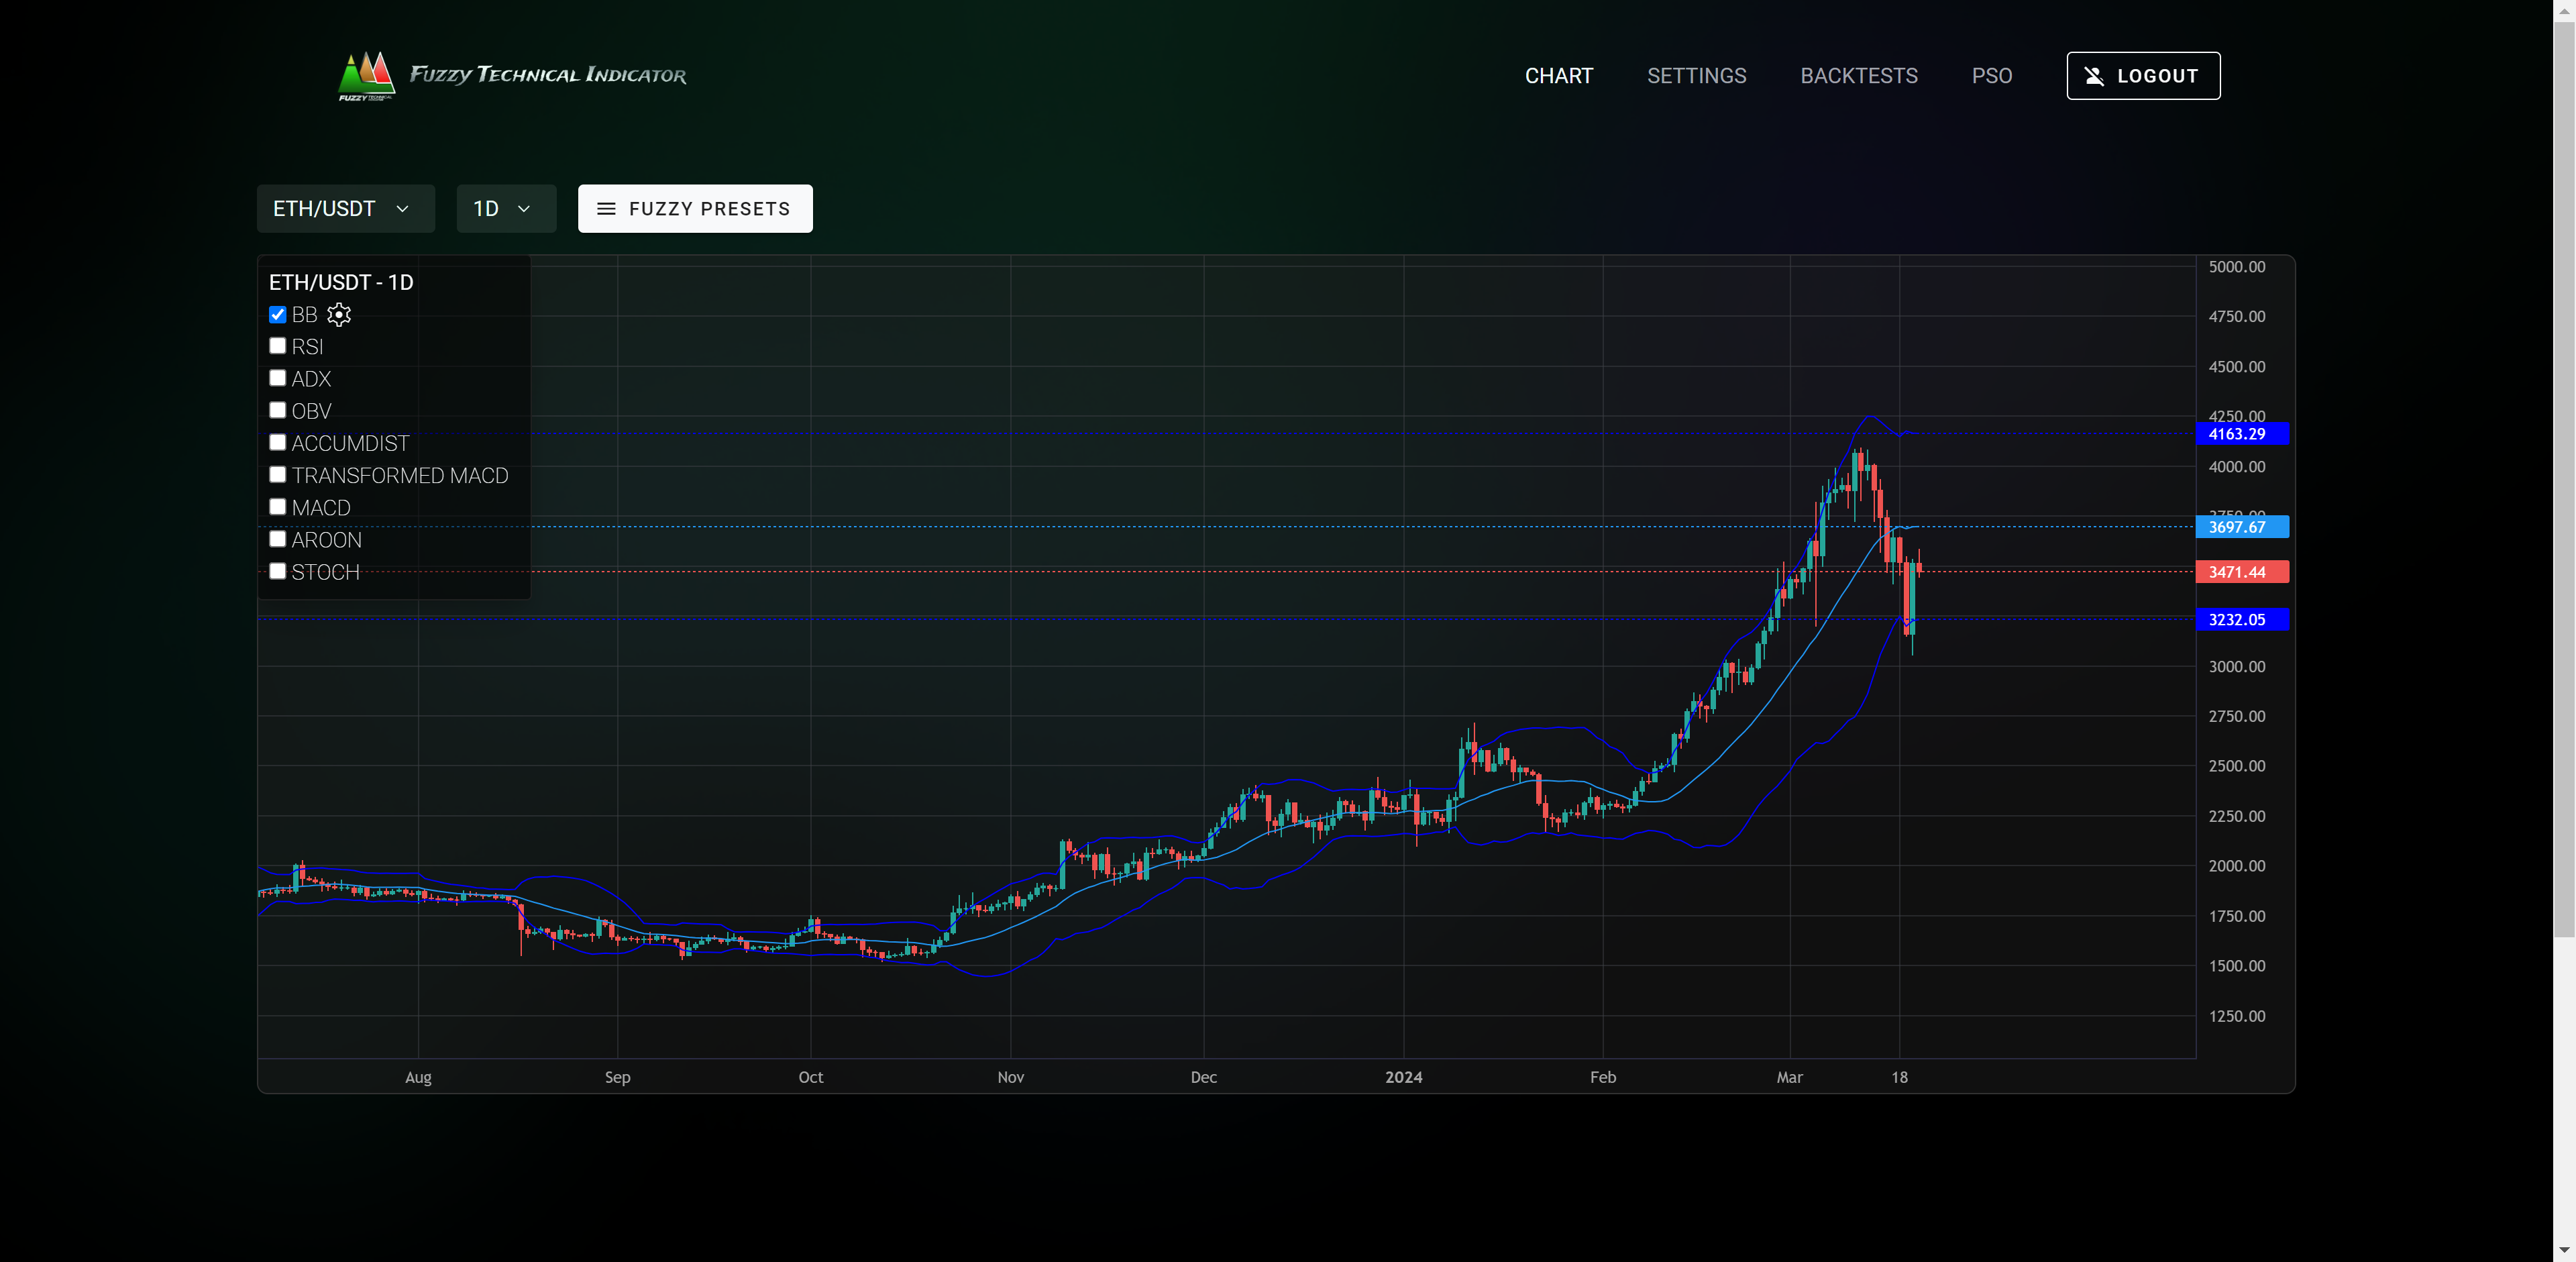
\includegraphics[width=\textwidth]{images/web-tuts/chart-ohlc.PNG}
    \caption{เว็บแอปพลิเคชัน หน้า Chart}
    \label{fig:chart-ohlc}
\end{figure}
\FloatBarrier
โดยผู้ใช้สามารถปรับเปลี่ยน Symbol และ Interval เป็นแบบอื่นได้ โดยการกดเลือกที่ Dropdown ดังรูป \ref{fig:chart-symbol-dd} และ \ref{fig:chart-interval-dd}
\begin{figure}[ht]
    \centering
    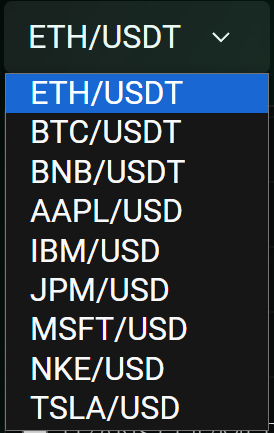
\includegraphics[scale=0.75]{images/web-tuts/chart-symbol-dd.PNG}
    \caption{Dropdown สำหรับการเปลี่ยน Symbol}
    \label{fig:chart-symbol-dd}
\end{figure}
\begin{figure}[ht]
    \centering
    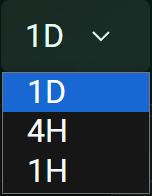
\includegraphics[scale=0.75]{images/web-tuts/chart-interval-dd.PNG}
    \caption{Dropdown สำหรับการเปลี่ยน Interval}
    \label{fig:chart-interval-dd}
\end{figure}
\FloatBarrier
ผู้ใช้สามารถเปิดใช้งานตัวชี้วัดทางเทคนิคพื้นฐานที่มีให้โดยการติ๊กที่ Box หน้าชื่อตัวชี้วัด ดังรูป \ref{fig:chart-indicators-selector}
\begin{figure}[ht]
    \centering
    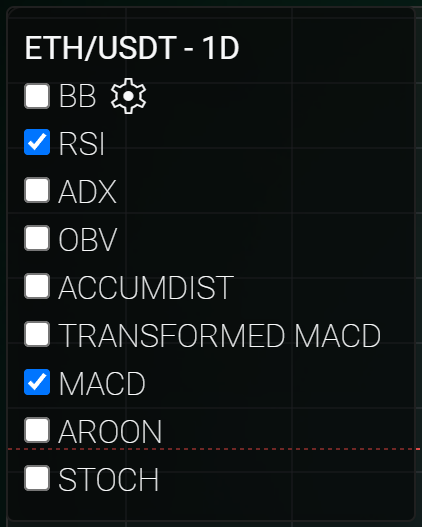
\includegraphics[scale=0.5]{images/web-tuts/chart-indicator-selector.PNG}
    \caption{การเปิดใช้งานตัวชี้วัดทางเทคนิคพื้นฐาน}
    \label{fig:chart-indicators-selector}
\end{figure}
\FloatBarrier
หลังจากเปิดใช้งานตัวชี้วัดทางเทคนิคจะแสดงกราฟผลลัพธ์ที่ได้ด้านล่างกราฟตลาดดังรูป \ref{fig:chart-indicator-on} และผู้ใช้สามารถปรับการตั้งค่าของตัวชี้วัดทางเทคนิคนั้นๆได้โดยกดที่รูปเฟืองจะแสดง Dialog การตั้งค่าขึ้นดังรูป \ref{fig:chart-indicator-setting}
\begin{figure}[ht]
    \centering
    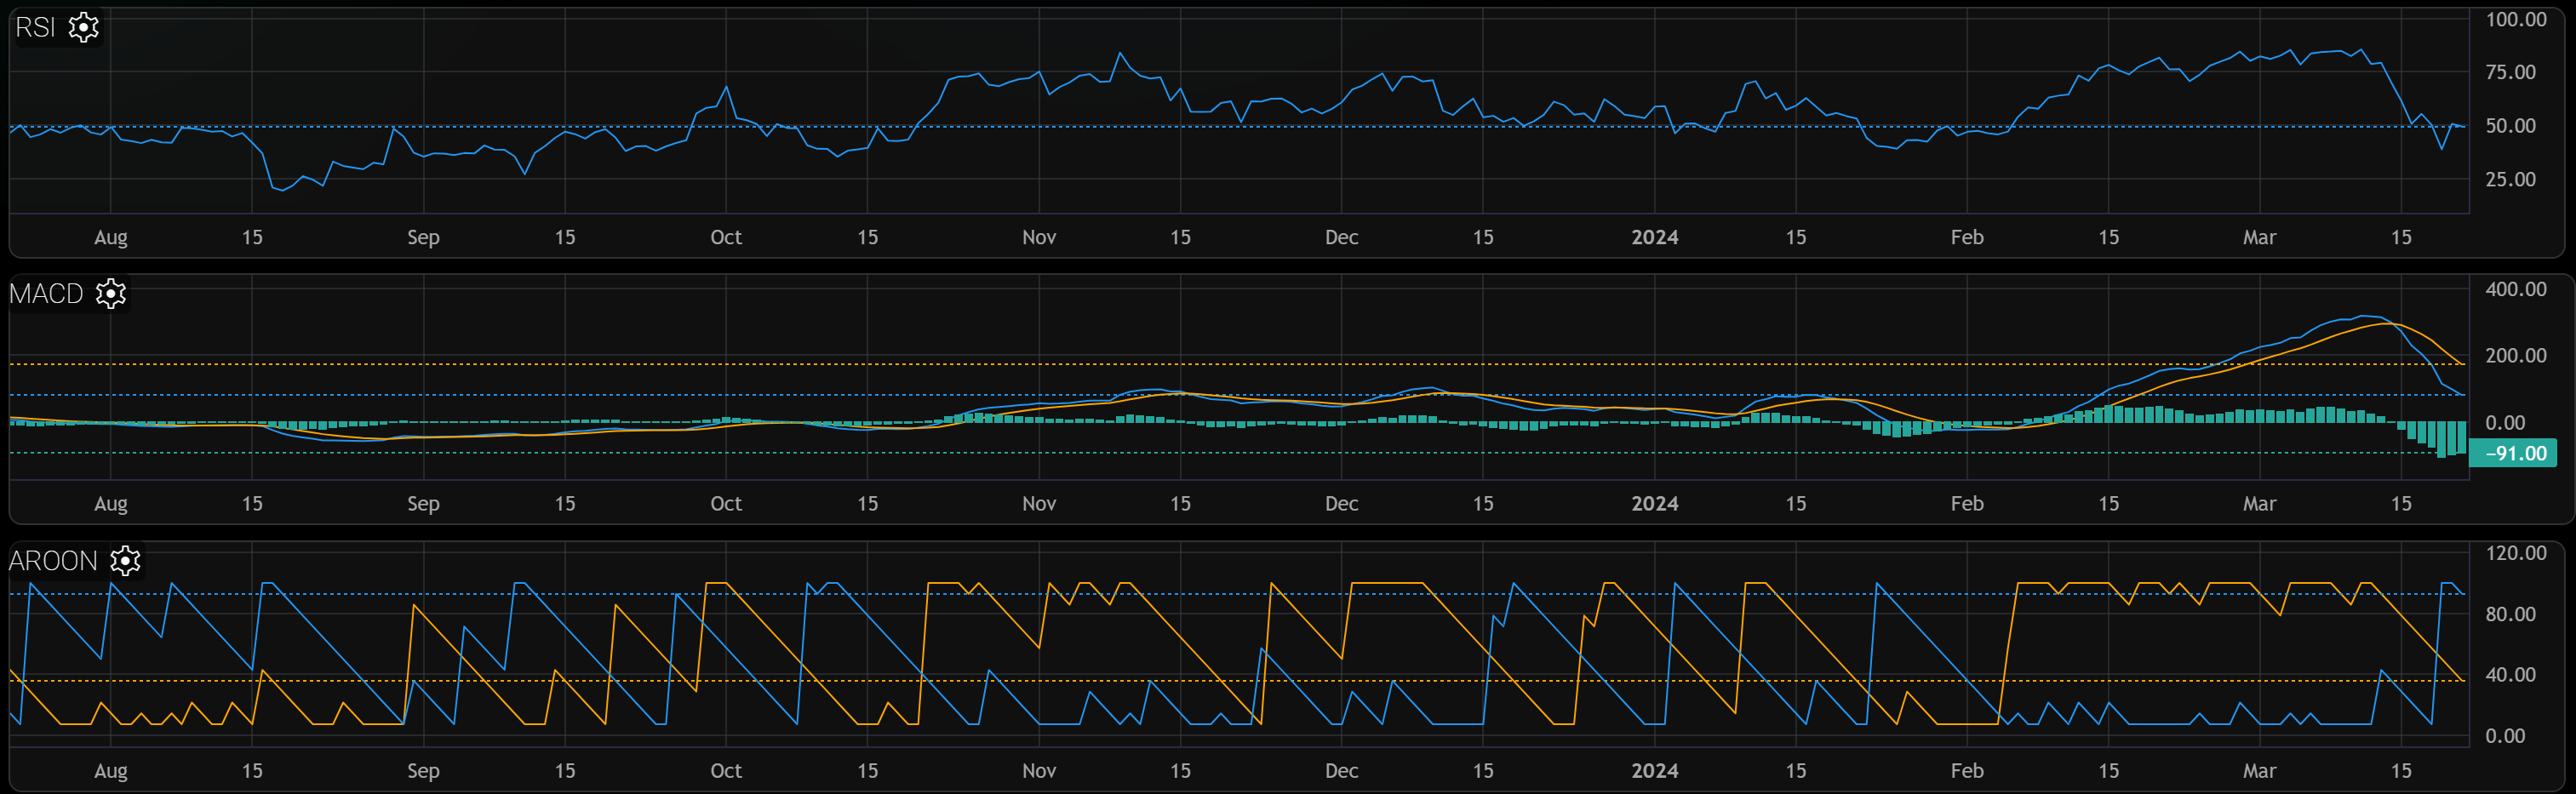
\includegraphics[width=\textwidth]{images/web-tuts/chart-indicator-on.PNG}
    \caption{กราฟแสดงผลลัพธ์ตัวชี้วัดทางเทคนิค RSI, MACD, AROON}
    \label{fig:chart-indicator-on}
\end{figure}
\begin{figure}[ht]
    \centering
    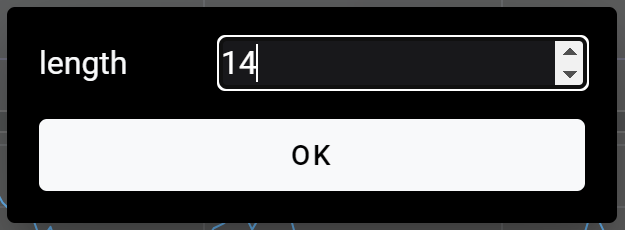
\includegraphics[scale=0.5]{images/web-tuts/chart-indicator-setting.PNG}
    \caption{Dialog สำหรับตั้งค่าตัวชี้วัดทางเทคนิค RSI}
    \label{fig:chart-indicator-setting}
\end{figure}
\FloatBarrier
และส่วนสุดท้ายคือการเปิดใช้งานตัวชี้วัดทางเทคนิคจากระบบ Fuzzy โดยกดที่ปุ่ม FUZZY PRESETS จะแสดง Dialog สำหรับการเลือกเปิดใช้งานตัวชี้วัด Fuzzy ตาม Presets ต่างๆที่เราสร้างไว้ ดังรูป \ref{fig:chart-fuzzypreset-selector} และ \ref{fig:chart-fuzzy-on}
\begin{figure}[ht]
    \centering
    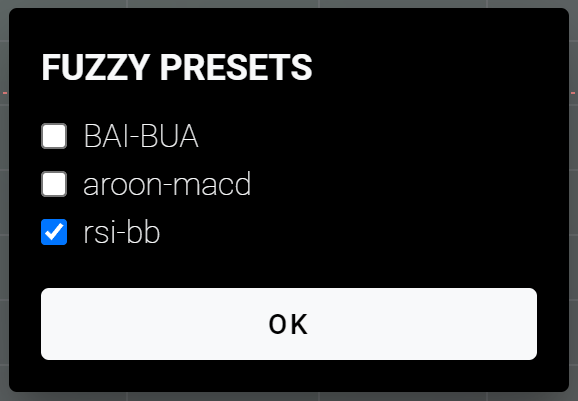
\includegraphics[scale=0.5]{images/web-tuts/chart-fuzzypreset-selector.PNG}
    \caption{Dialog สำหรับการเลือกเปิดใช้งานตัวชี้วัด Fuzzy จาก Preset}
    \label{fig:chart-fuzzypreset-selector}
\end{figure}
\begin{figure}[h]
    \centering
    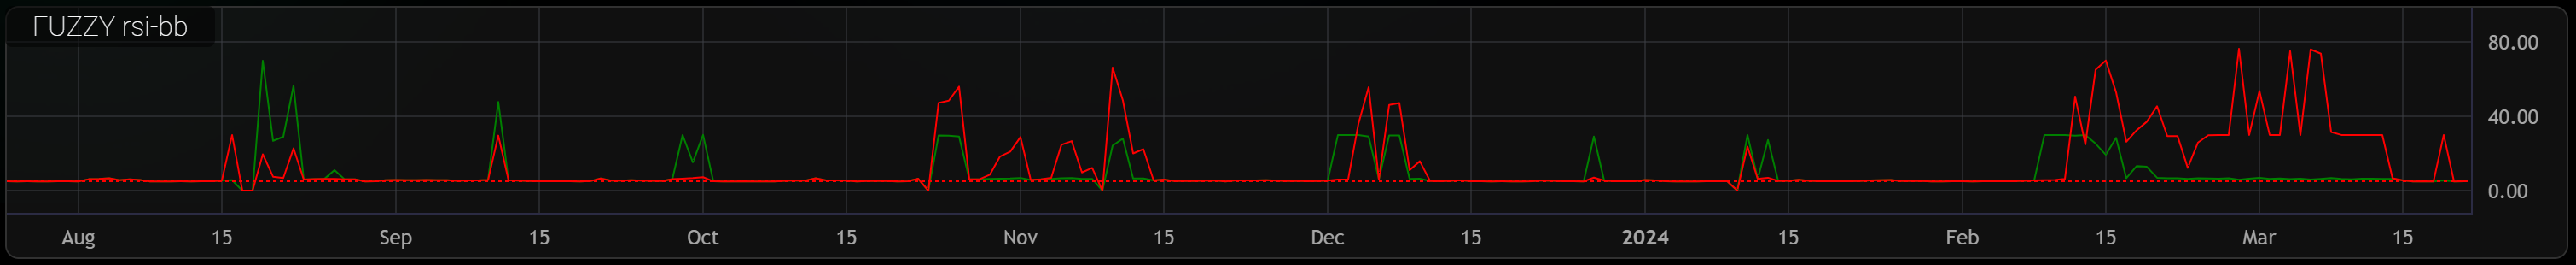
\includegraphics[width=\textwidth]{images/web-tuts/chart-fuzzy-on.PNG}
    \caption{กราฟแสดงผลลัพธ์ตัวชี้วัดทางเทคนิคที่ได้จากระบบ Fuzzy}
    \label{fig:chart-fuzzy-on}
\end{figure}
\FloatBarrier

\subsubsection{การใช้งานหน้า Settings}
หน้า Settings จะใช้สำหรับการ สร้าง/แก้ไข/ลบ Fuzzy Preset ของเราโดยเมื่อเข้ามาแล้วจะแสดง Fuzzy Preset ทั้งหมดของเราที่มีดังรูป \ref{fig:settings-presets}
\begin{figure}[ht]
    \centering
    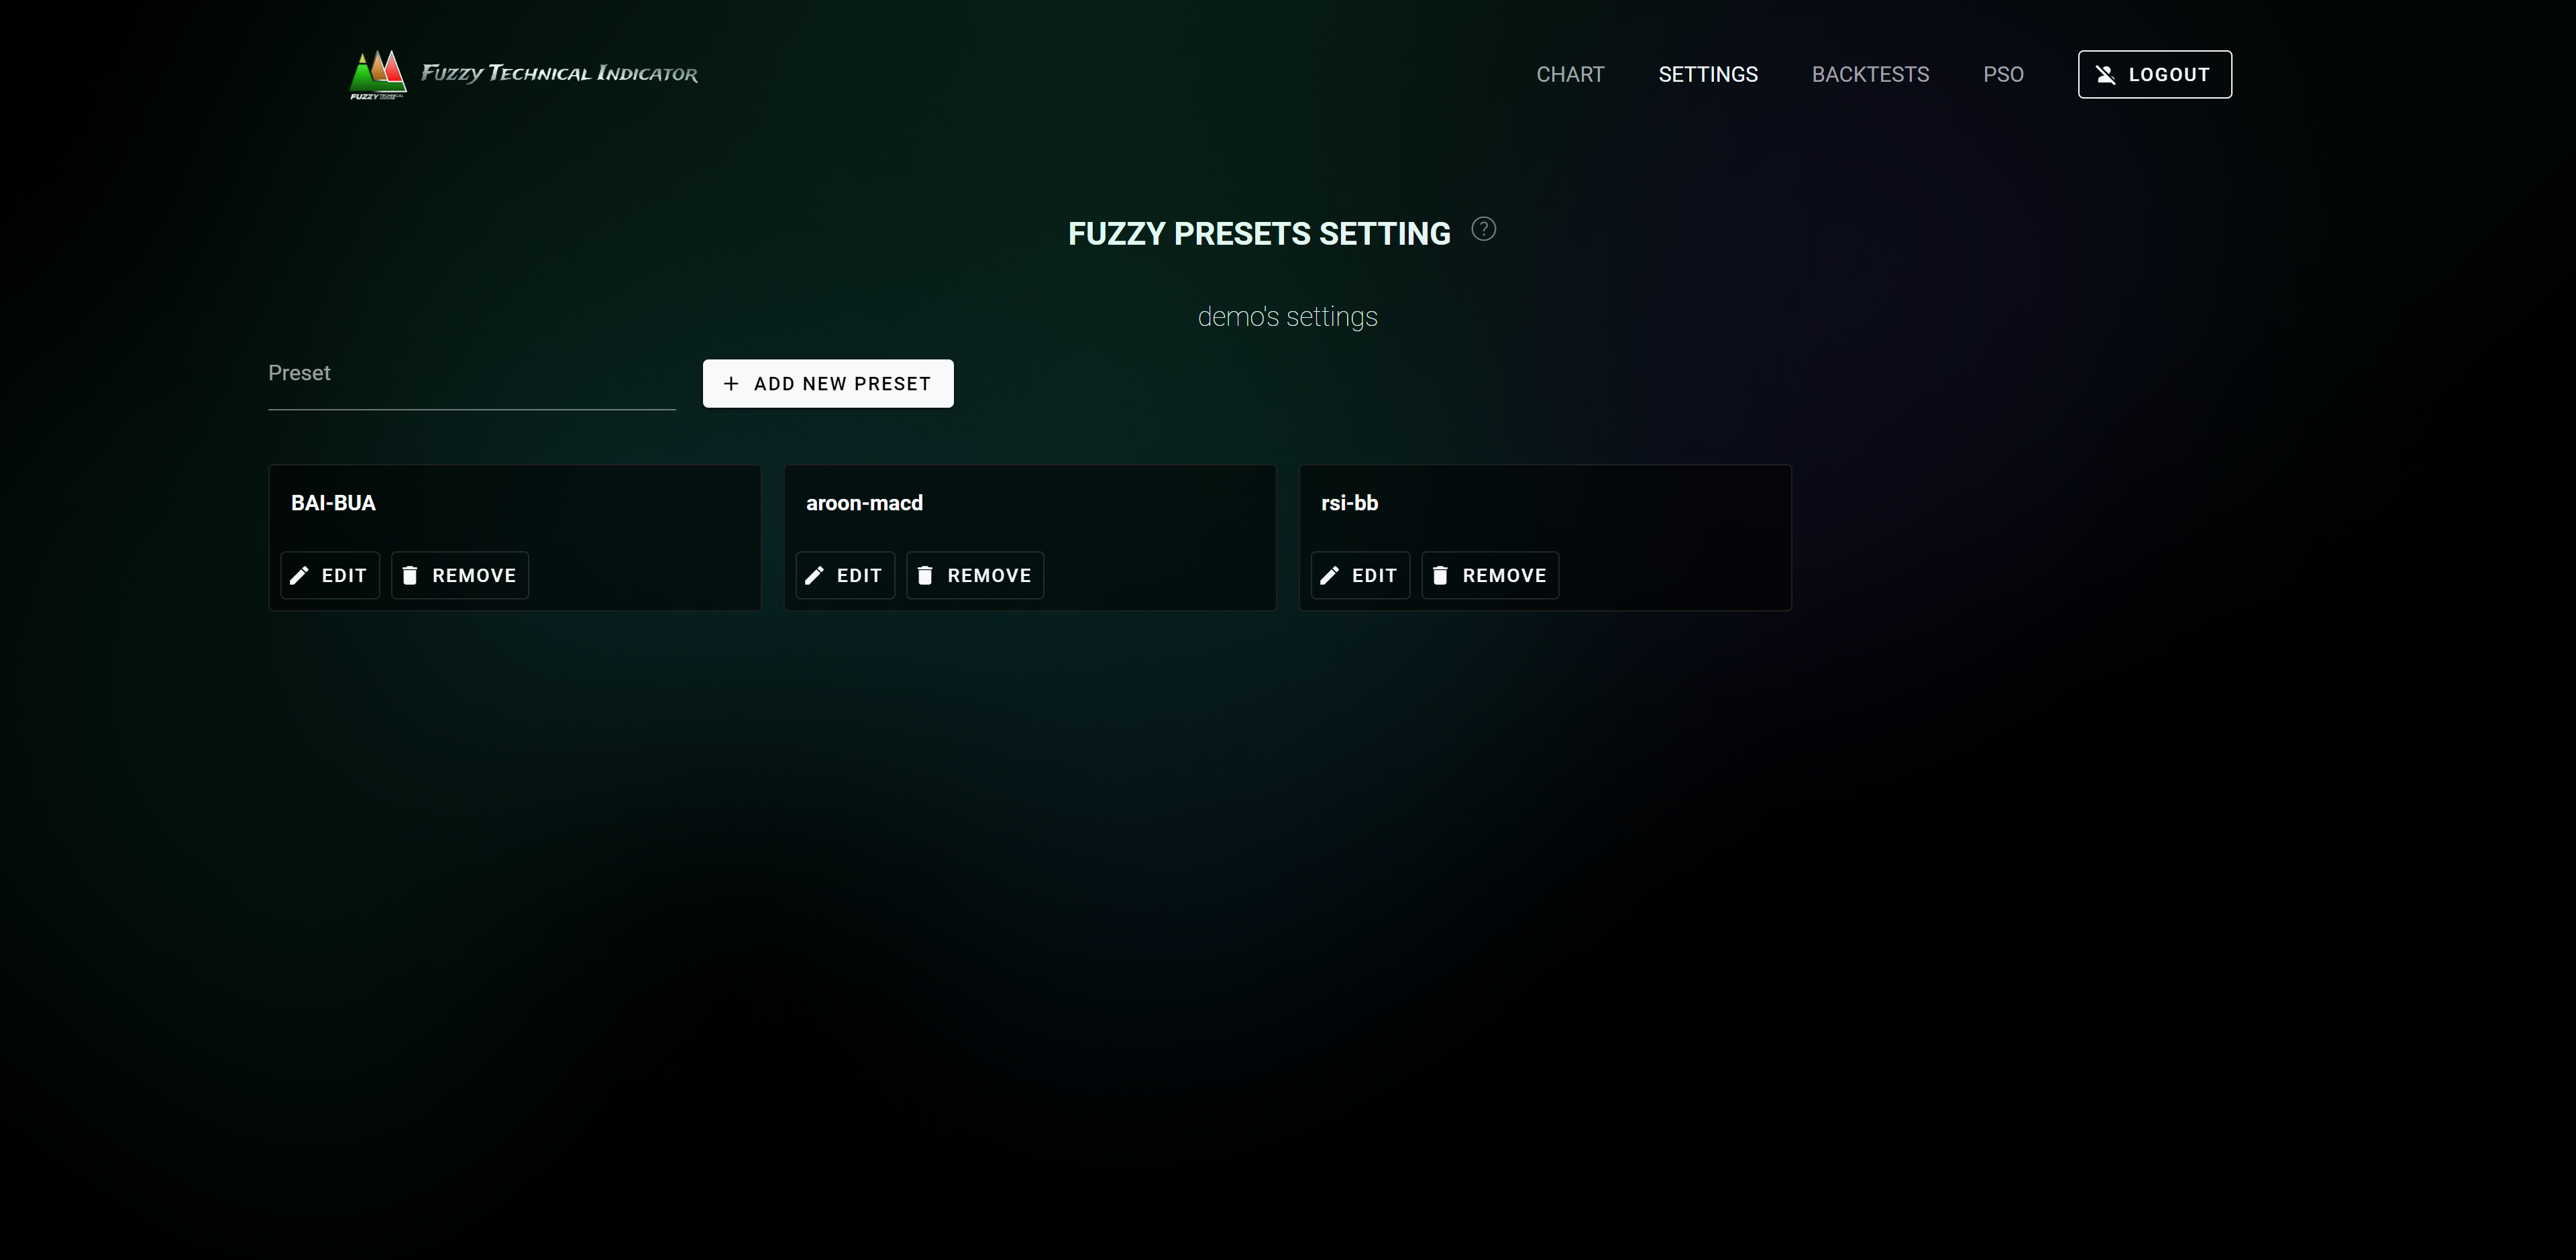
\includegraphics[width=\textwidth]{images/web-tuts/settings-presets.PNG}
    \caption{เว็บแอปพลิเคชัน หน้า Settings}
    \label{fig:settings-presets}
\end{figure}
\FloatBarrier
ในการสร้าง Fuzzy Preset ใหม่ให้ทำการพิมพ์ชื่อลงในช่อง Preset และกดปุ่ม ADD NEW PRESET โดยจะทำการสร้างและนำพาไปยังหน้าตั้งค่าตัวแปรภาษาและกฏฟัซซีดังรูป \ref{fig:settings-new-preset}
\begin{figure}[ht]
    \centering
    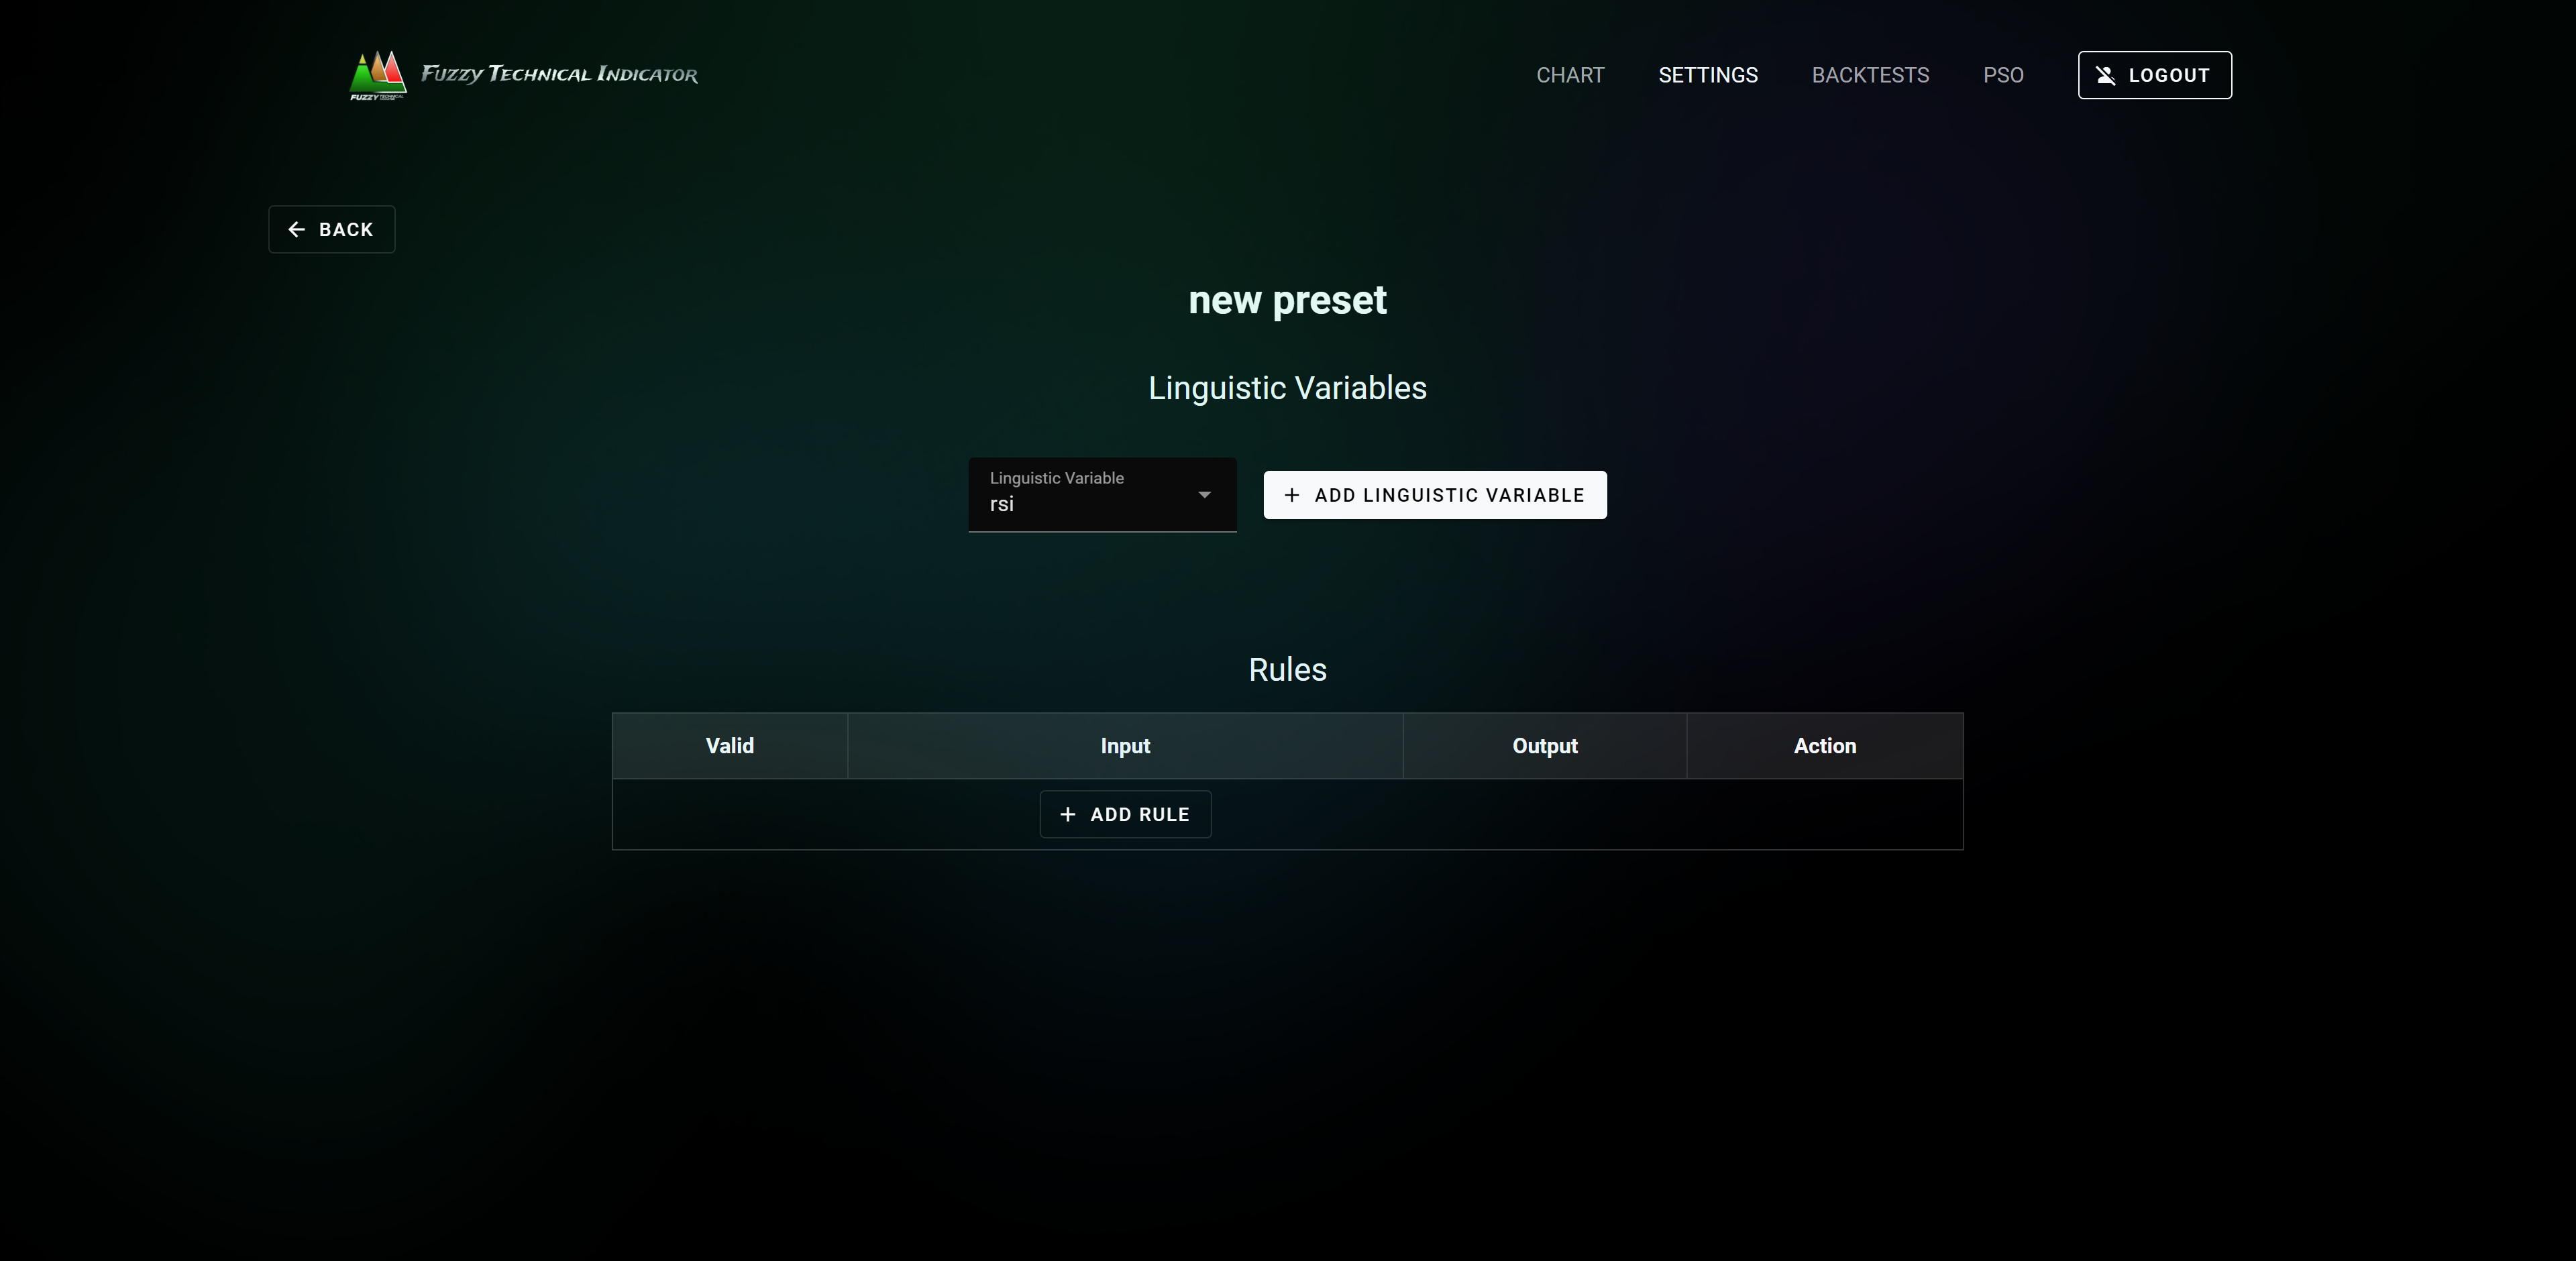
\includegraphics[width=\textwidth]{images/web-tuts/settings-new-preset.PNG}
    \caption{Settings ในส่วนหน้าตั้งค่าตัวแปรทางภาษาและกฏฟัซซี}
    \label{fig:settings-new-preset}
\end{figure}
\FloatBarrier
โดยเริ่มแรกใน Preset ที่สร้างใหม่จะยังไม่มีตัวแปรทางภาษาและกฏ จะต้องทำการเพิ่มโดยใช้ตัวเลือก Dropdown ในการเลือกตัวชี้วัดพื้นฐานเป็นตัวแปรทางภาษา Input และเลือก custom เพื่อสร้างตัวแปรทางภาษา Output โดยจะต้องใส่ชื่อ long/short ดังรูป \ref{fig:settings-lingvars-dd} และ \ref{fig:settings-lingvars-custom}
\begin{figure}[ht]
    \centering
    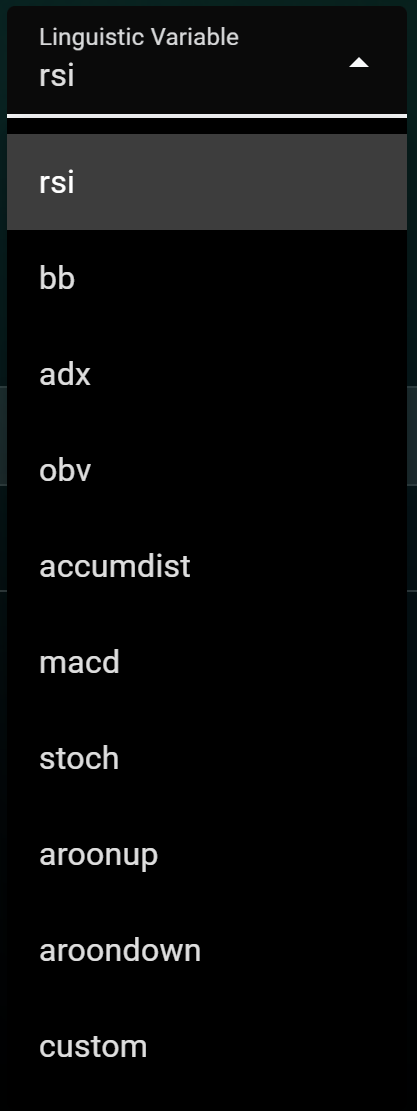
\includegraphics[scale=0.5]{images/web-tuts/settings-lingvars-dd.PNG}
    \caption{Dropdown สำหรับเลือกตัวชี้วัดพื้นฐานเป็นตัวแปรทางภาษา}
    \label{fig:settings-lingvars-dd}
\end{figure}
\begin{figure}[ht]
    \centering
    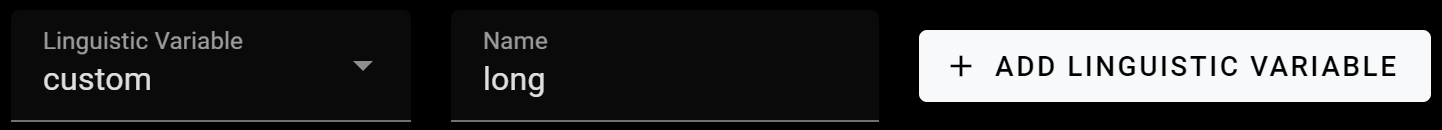
\includegraphics[width=\textwidth]{images/web-tuts/settings-lingvars-custom.PNG}
    \caption{การเพิ่มตัวแปรทางภาษา Output}
    \label{fig:settings-lingvars-custom}
\end{figure}
\FloatBarrier
และเมื่อทำการกดปุ่ม ADD LINGUISTIC VARIABLE แล้วจะมีกราฟแสดงในส่วนของรูปร่างของตัวแปรทางภาษาดังรูป \ref{fig:settings-rsi-init} ซึ่งจะยังไม่มีข้อมูลผู้ใช้งานต้องทำการปรับเปลี่ยนในส่วนของ Universe และ Shapes ของตัวแปรทางภาษาโดยจะสามารถเพิ่ม Shape ได้ 2 แบบคือ Triangle, Trapezoid ดังรูป \ref{fig:settings-lingvar-editor}, \ref{fig:settings-lingvar-shapes-dd}
\begin{figure}[ht]
    \centering
    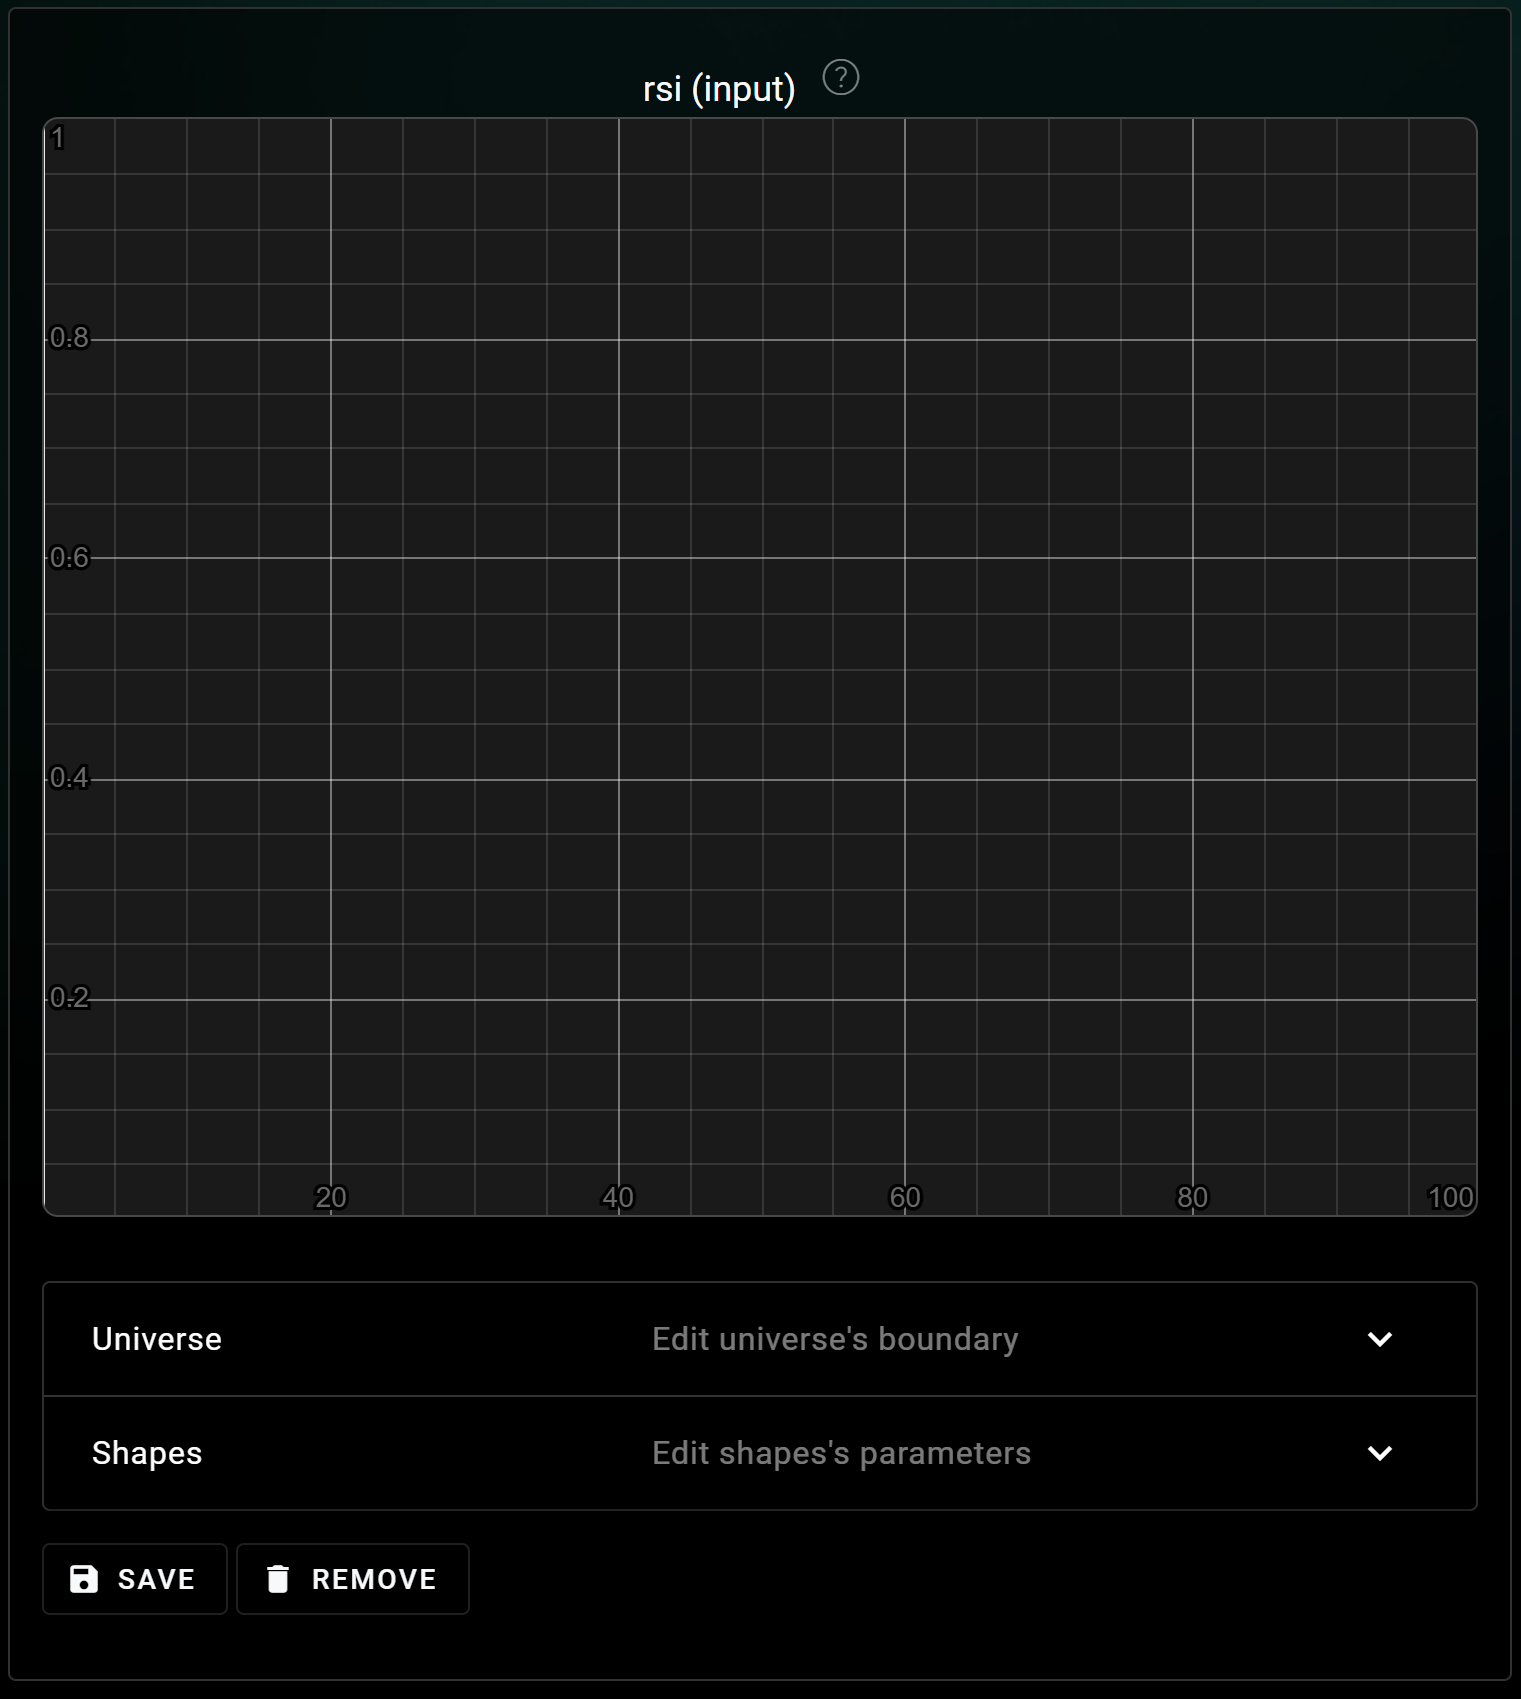
\includegraphics[scale=0.5]{images/web-tuts/settings-rsi-init.PNG}
    \caption{กราฟตัวแปรทางภาษา Input RSI ที่ยังไม่ได้ตั้งค่า}
    \label{fig:settings-rsi-init}
\end{figure}
\begin{figure}[ht]
    \centering
    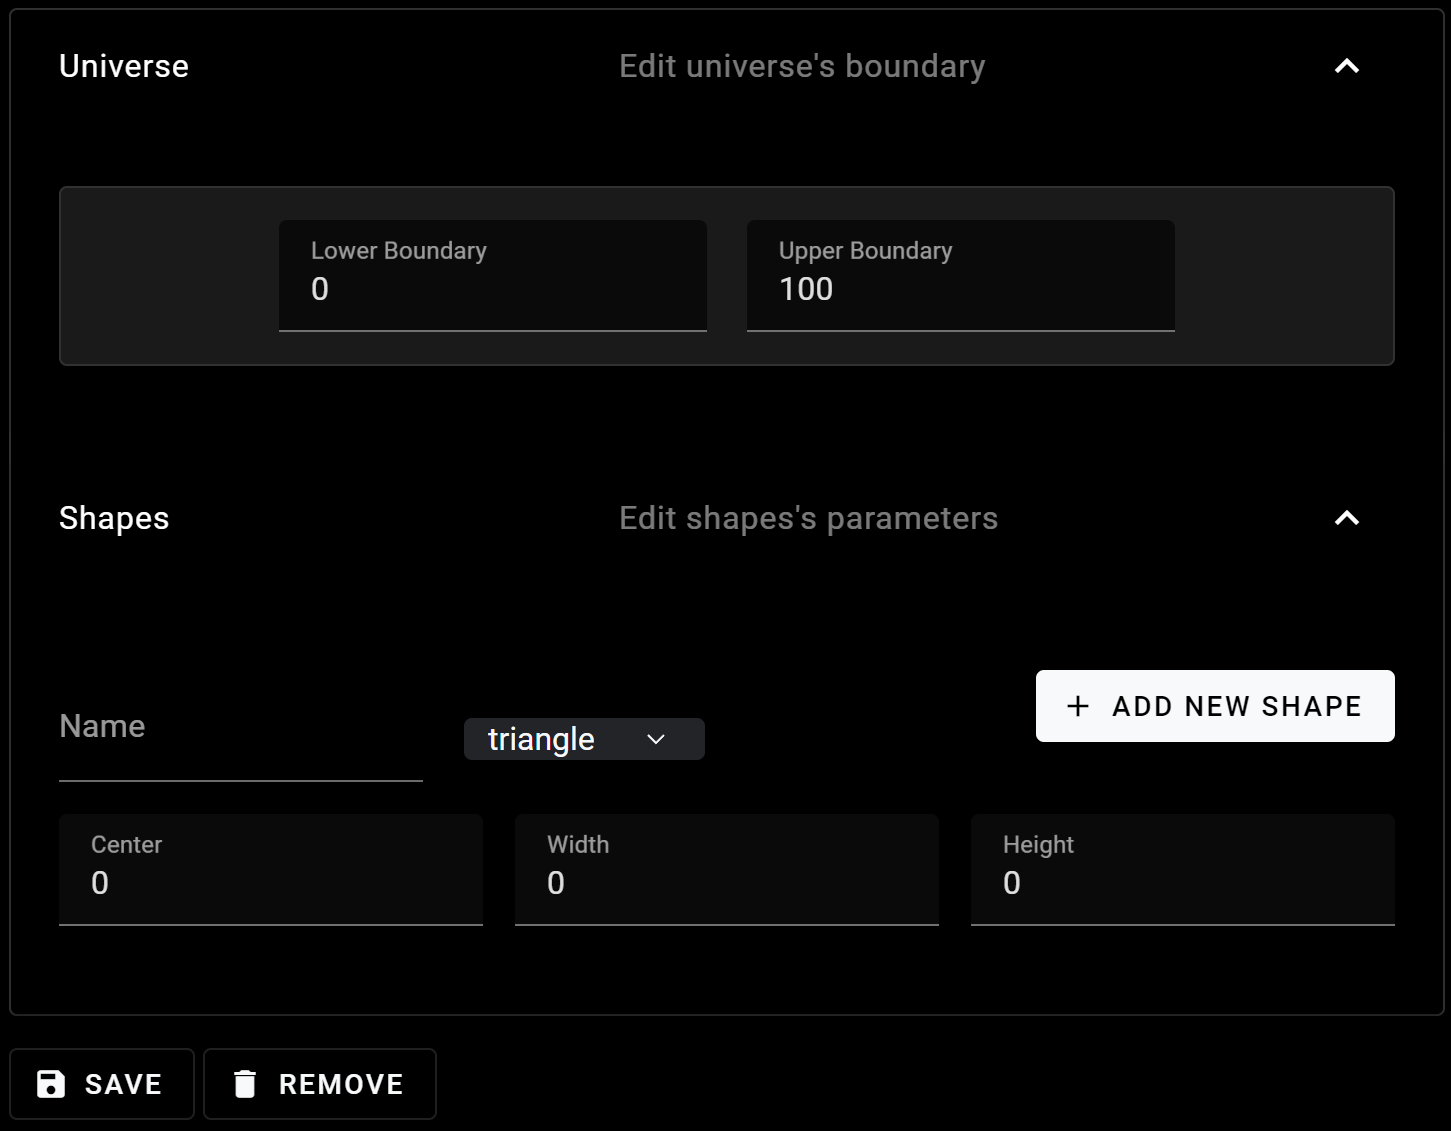
\includegraphics[scale=0.5]{images/web-tuts/settings-lingvar-editor.PNG}
    \caption{เมนูการตั้งค่า Universe และ Shapes ของตัวแปรทางภาษา}
    \label{fig:settings-lingvar-editor}
\end{figure}
\begin{figure}[ht]
    \centering
    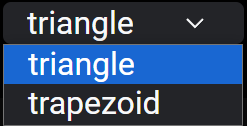
\includegraphics[scale=0.75]{images/web-tuts/settings-lingvar-shapes-dd.PNG}
    \caption{Dropdown สำหรับการเลือกเพิ่ม Shape ในตัวแปรทางภาษา}
    \label{fig:settings-lingvar-shapes-dd}
\end{figure}
\FloatBarrier
โดยเมื่อทำการปรับเปลี่ยน Universe และ Shapes แล้วจะต้องทำการกดปุ่ม Save เพื่อบันทึกการเปลี่ยนแปลง หรือปุ่ม Remove เพื่อลบตัวแปรทางภาษาได้ โดยเมื่อทำการปรับเปลี่ยนแล้วจะได้ดังรูป \ref{fig:settings-lingvar-edited}
\begin{figure}[ht]
    \centering
    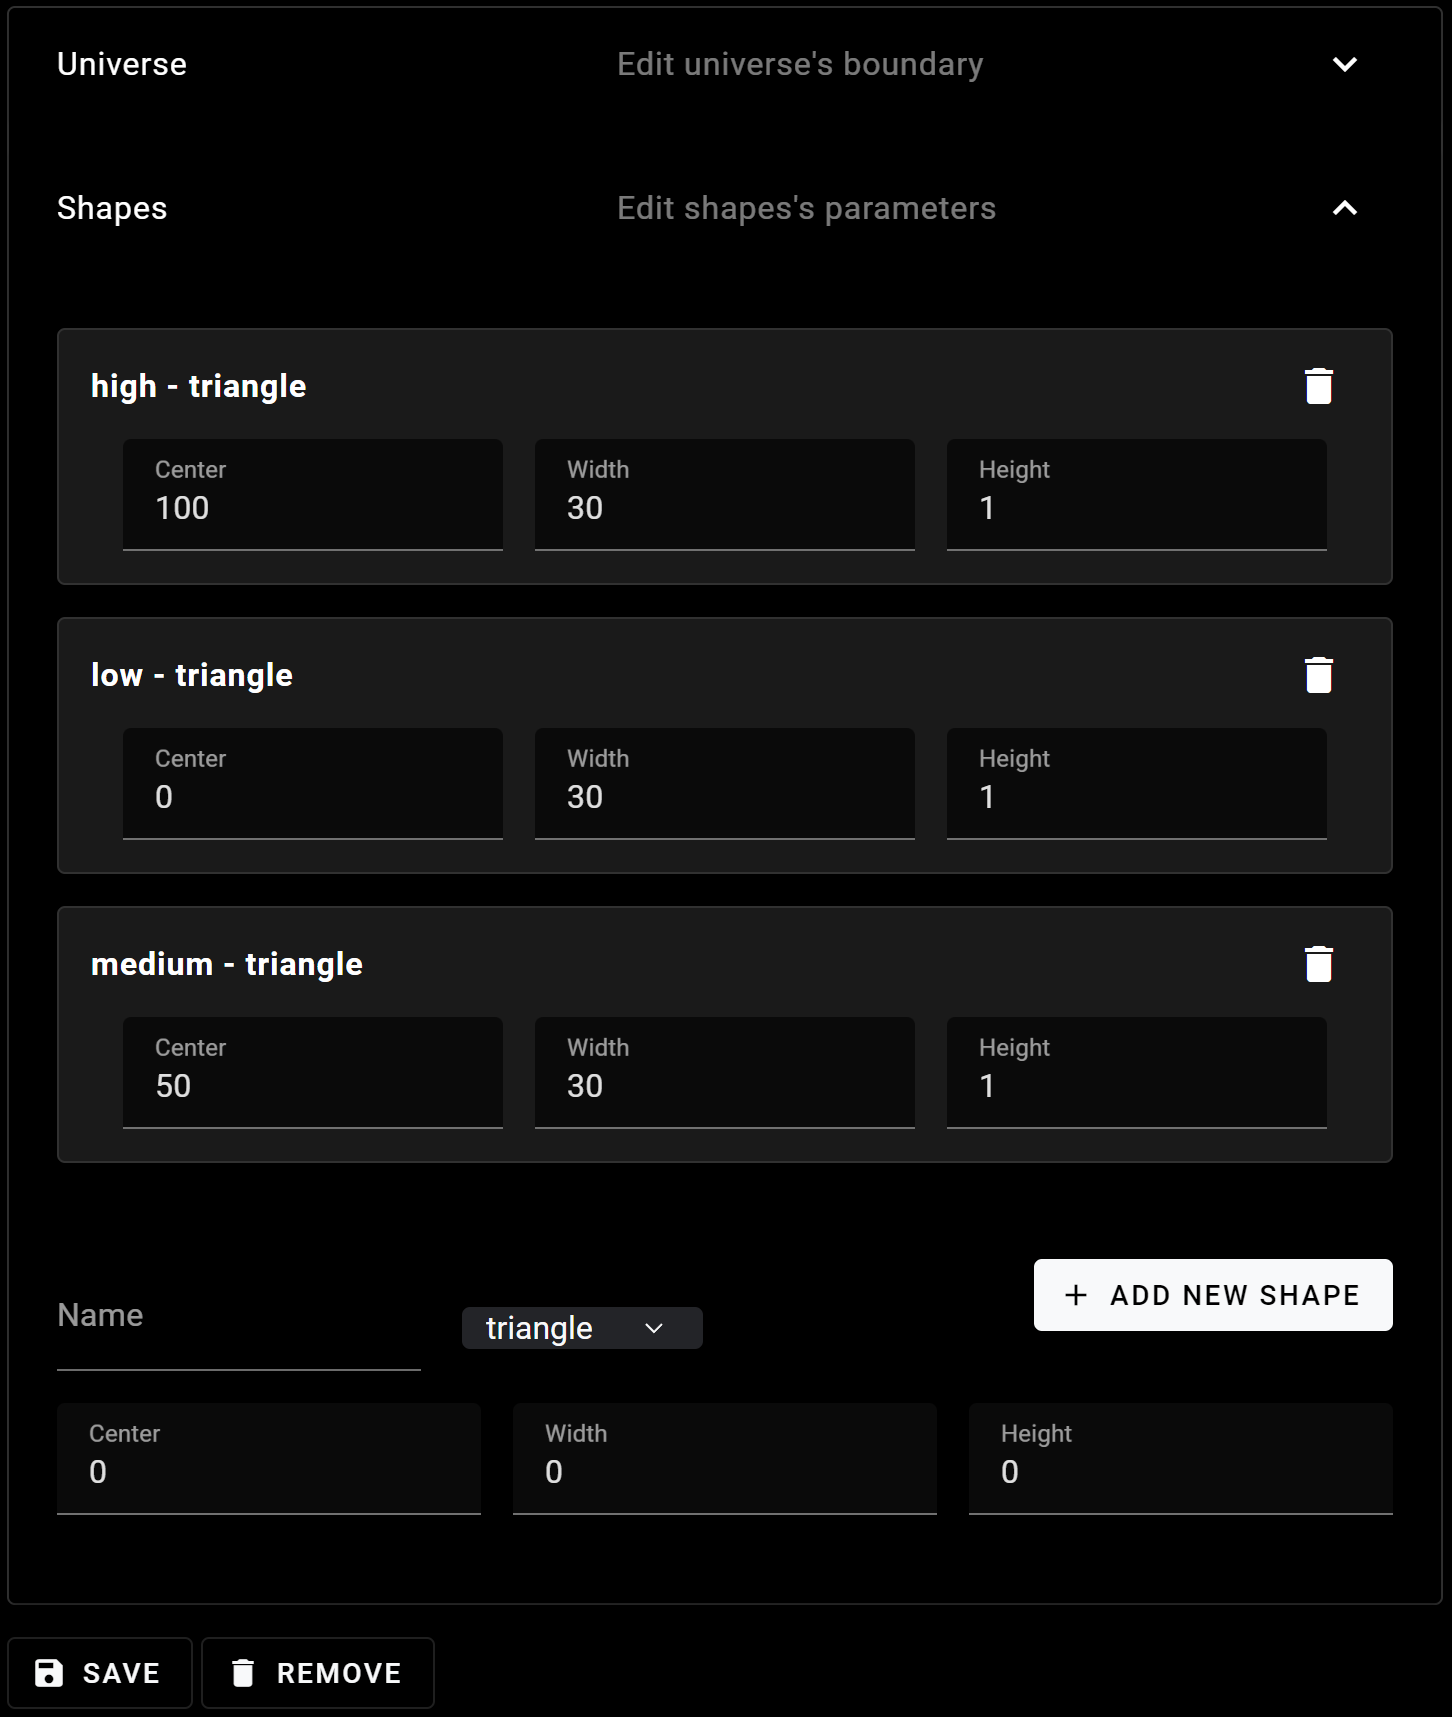
\includegraphics[scale=0.5]{images/web-tuts/settings-lingvar-edited.PNG}
    \caption{เมนู Universe และ Shapes เมื่อปรับตั้งค่าแล้ว}
    \label{fig:settings-lingvar-edited}
\end{figure}
\FloatBarrier
และกราฟจะแสดง Shapes ที่ผู้ใช้สร้างเข้าไปดังรูป \ref{fig:settings-lingvar-edited-graph}
\begin{figure}[ht]
    \centering
    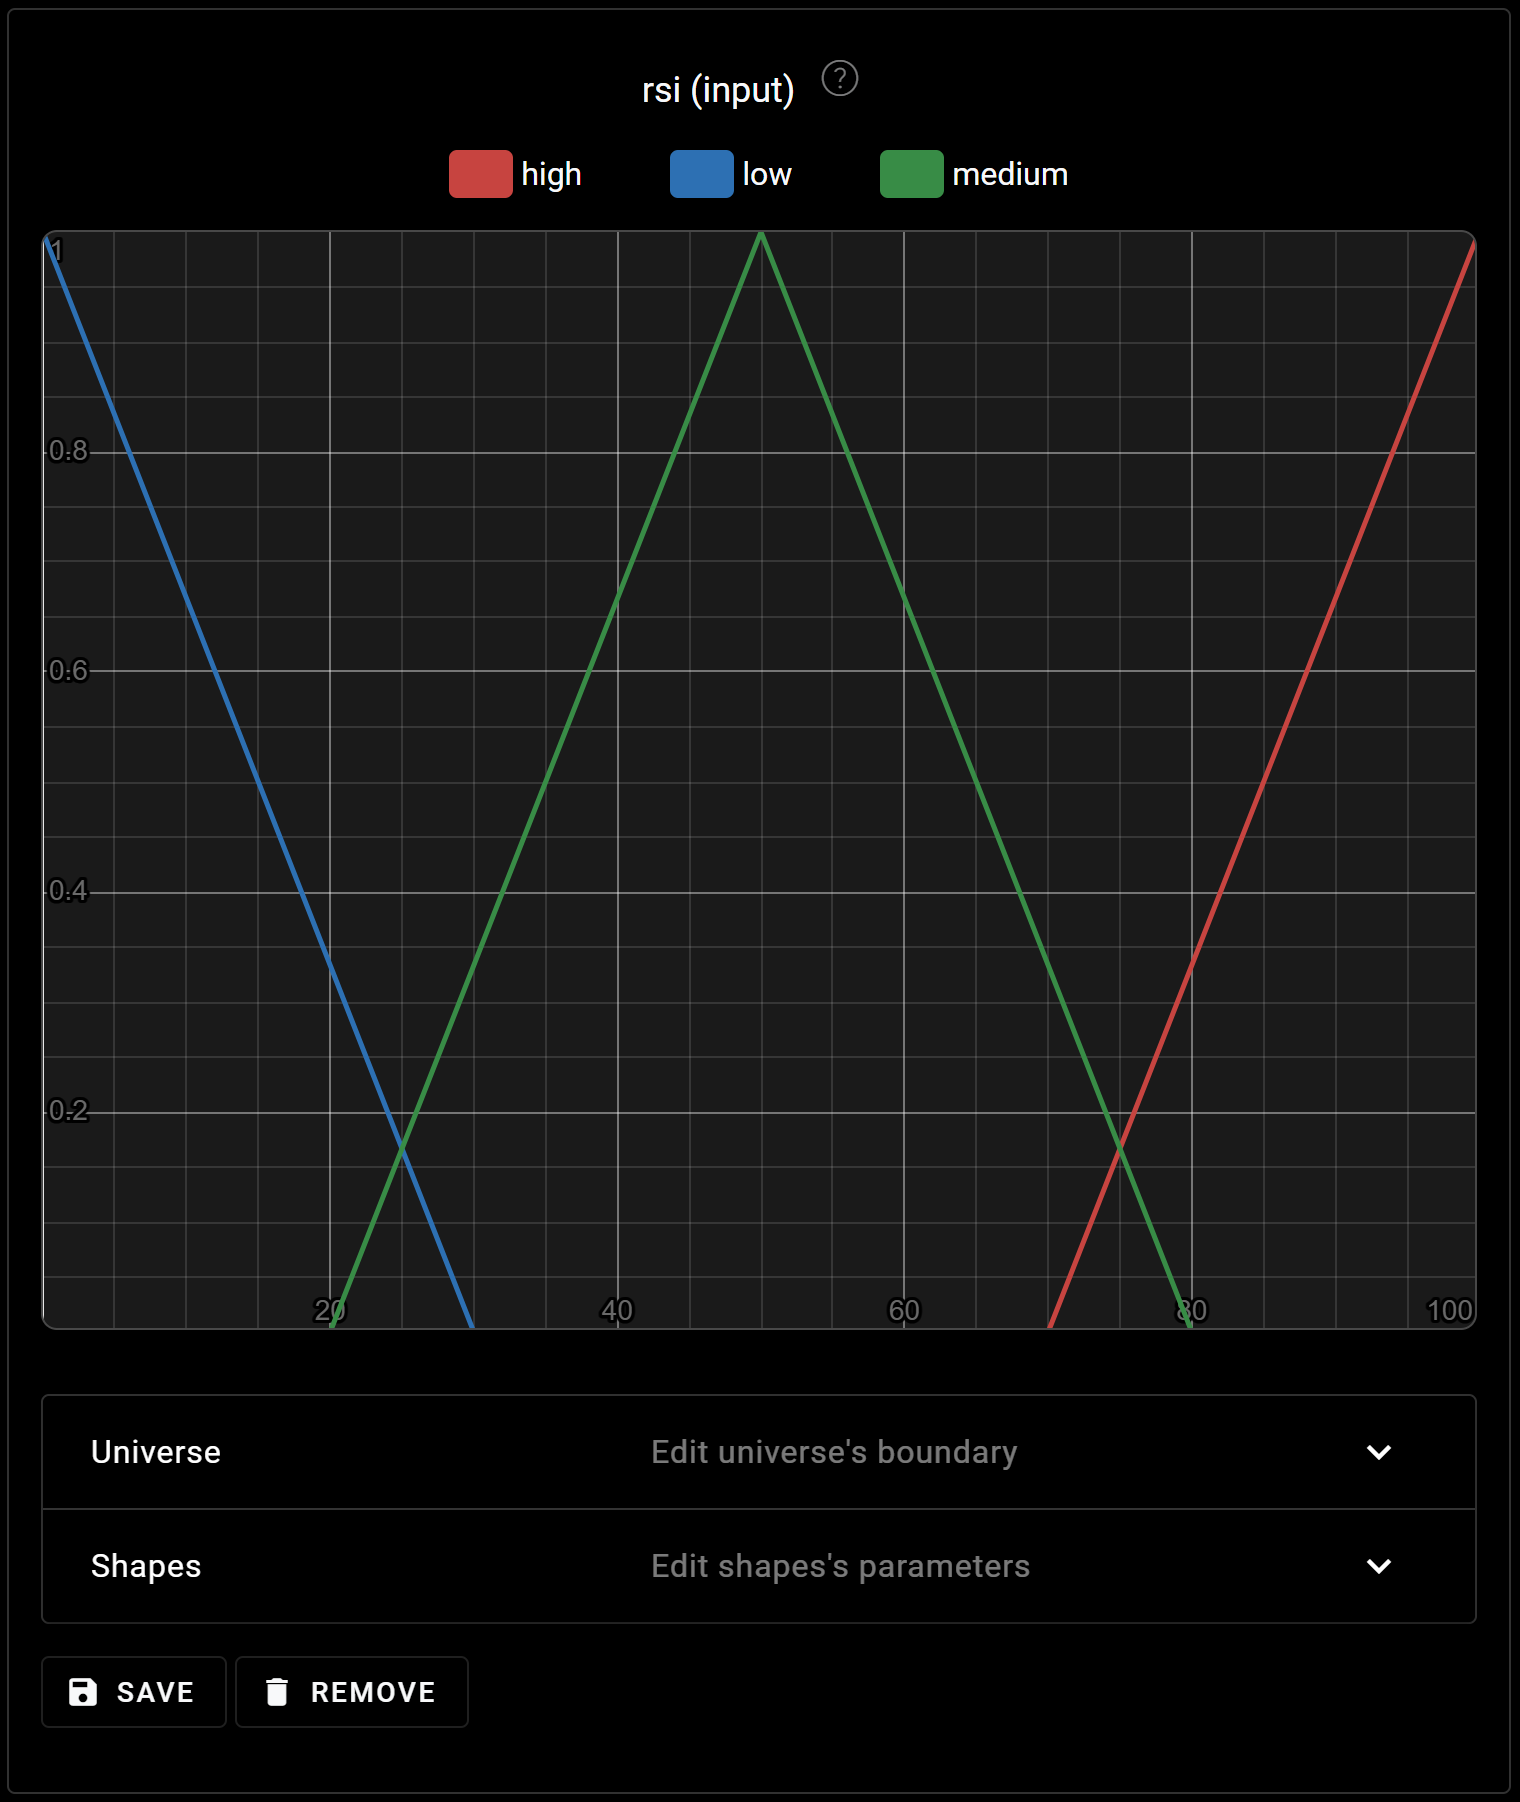
\includegraphics[scale=0.5]{images/web-tuts/settings-lingvar-edited-graph.PNG}
    \caption{กราฟตัวแปรทางภาษาเมื่อปรับตั้ง Universe และ Shapes แล้ว}
    \label{fig:settings-lingvar-edited-graph}
\end{figure}
\FloatBarrier
ในส่วนสุดท้ายจะเป็นการเพิ่มกฏฟัซซีโดยจะเพิ่มได้อย่างสมบูรณ์ก็ต่อเมื่อผู้ใช้งานทำการสร้างตัวแปรทางภาษาทั้ง Input และ Output แล้ว โดยจะสามารถเลือกระดับตัวแปรทางภาษาในแต่ละตัวแปรทางภาษา Input, Output และทำการกดปุ่ม ADD RULE เพื่อเพิ่มกฏ หากกฏที่เพิ่มสมบูรณ์ในคอลัมน์ Valid จะแสดงคำว่า true ด้านหน้ากฏนั้นๆ ดังรูป \ref{fig:settings-rules} และ \ref{fig:settings-rules-dd}
\begin{figure}[ht]
    \centering
    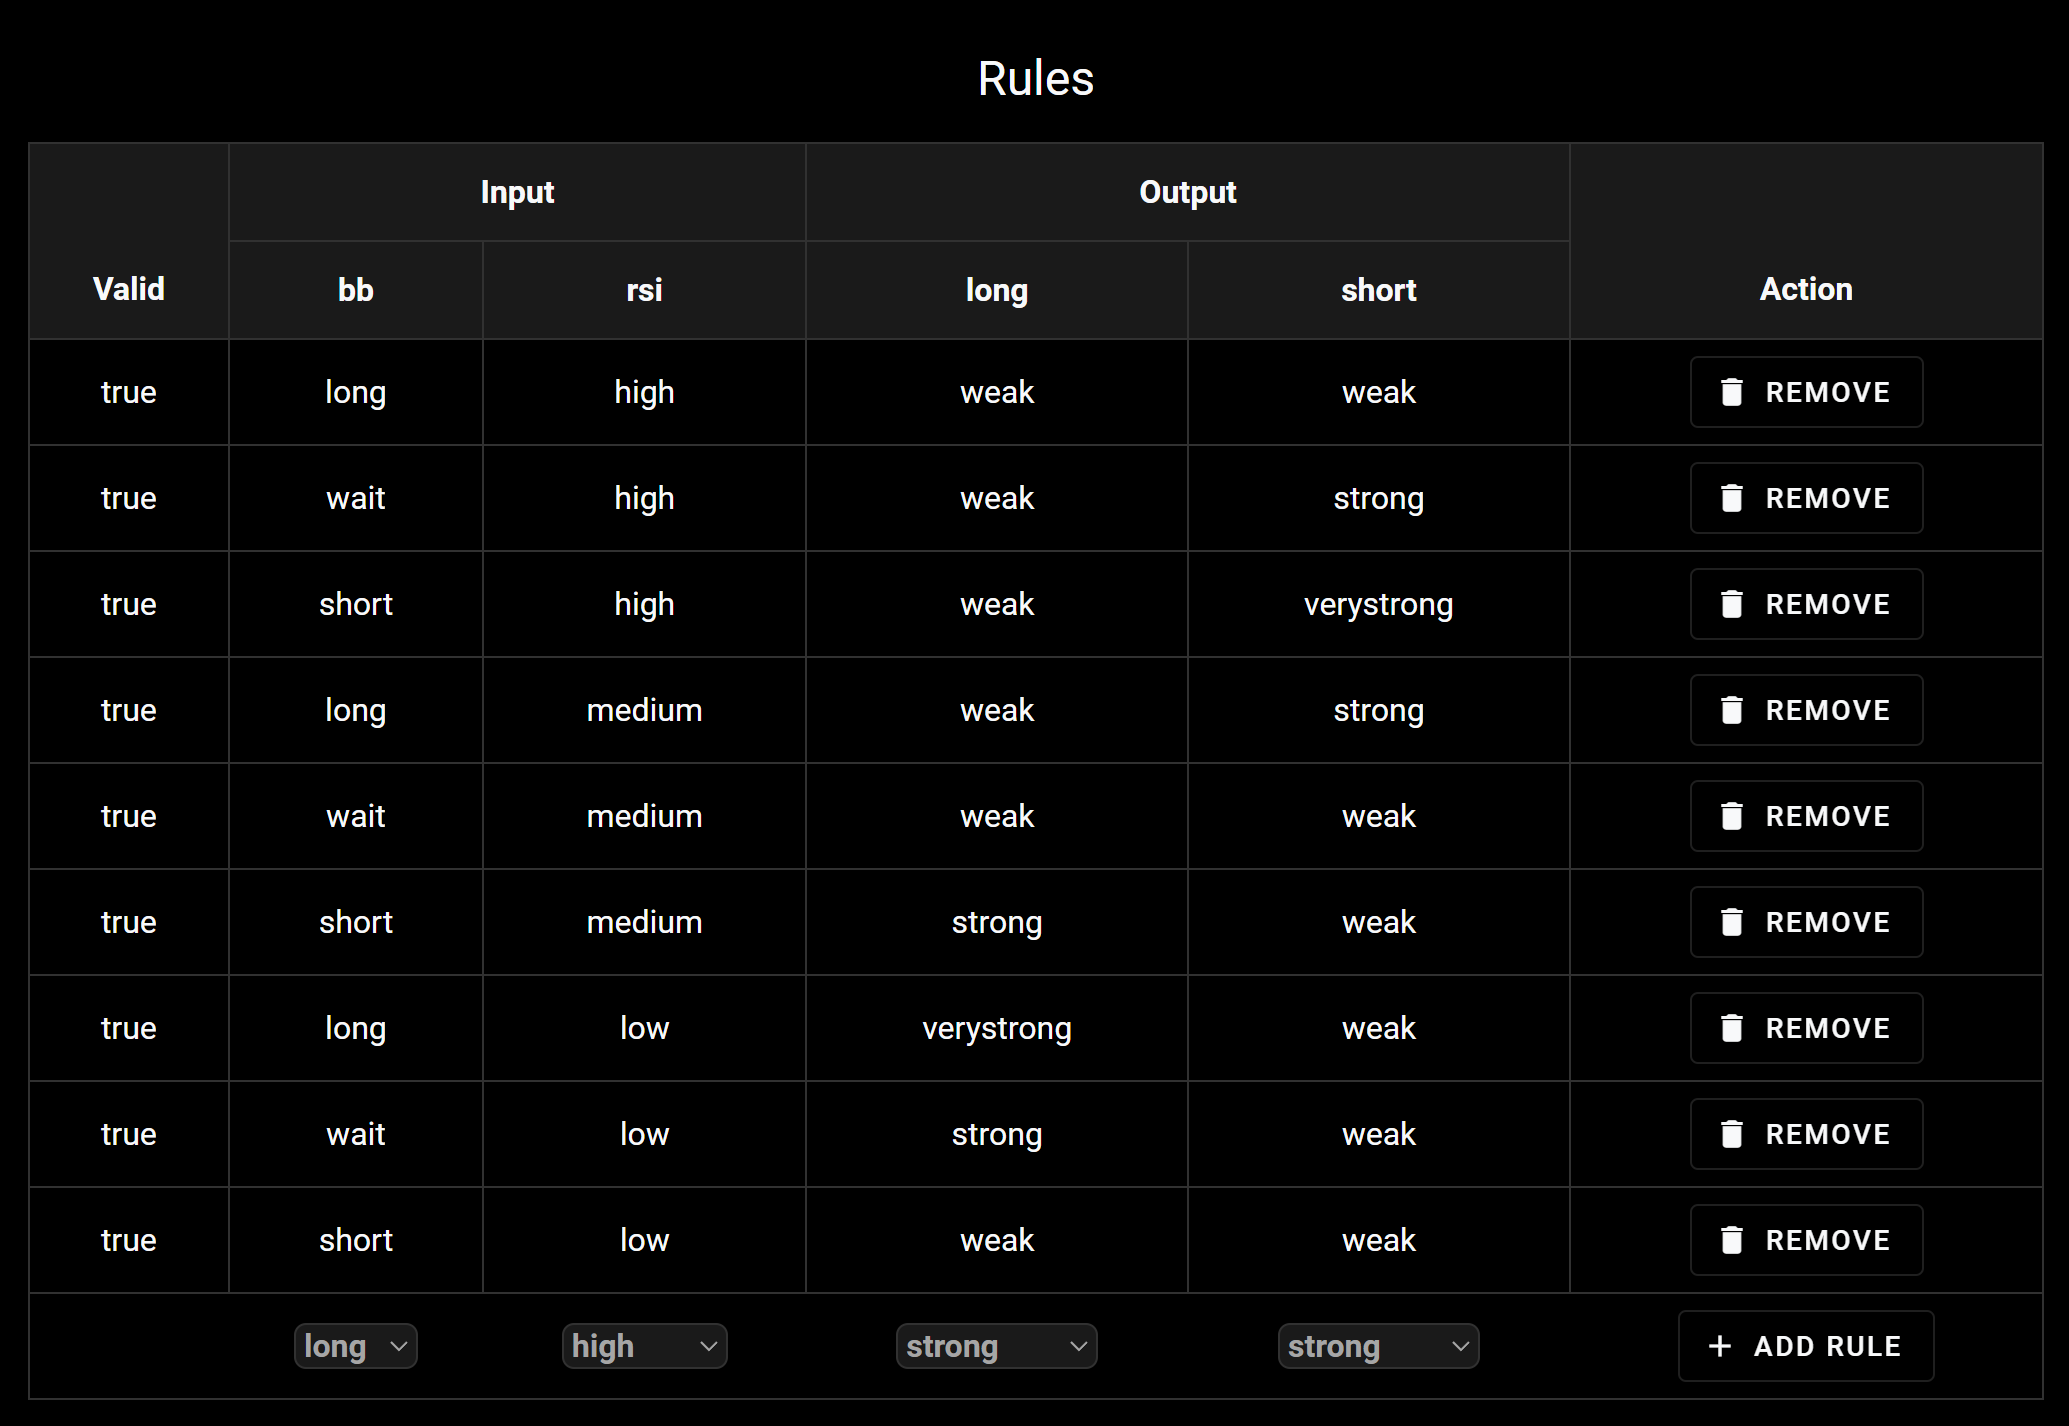
\includegraphics[width=\textwidth]{images/web-tuts/settings-rules.PNG}
    \caption{เมนู เพิ่ม/ลบ กฏฟัซซีใน Preset}
    \label{fig:settings-rules}
\end{figure}
\begin{figure}[ht]
    \centering
    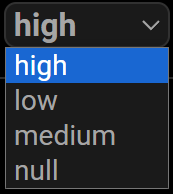
\includegraphics[scale=0.75]{images/web-tuts/settings-rules-dd.PNG}
    \caption{Dropdown การเลือกระดับตัวแปรทางภาษาตาม Shapes ที่ผู้ใช้งานสร้างไว้ในตัวแปรทางภาษานั้น}
    \label{fig:settings-rules-dd}
\end{figure}
\FloatBarrier

\subsubsection{การใช้งานหน้า Backtests}
หน้า Backtests จะใช้สำหรับการทดสอบกลยุทธ์ย้อนหลังบน Fuzzy Preset และดูผลลัพธ์การทดสอบ \ref{fig:backtest-no-result}
\begin{figure}[ht]
    \centering
    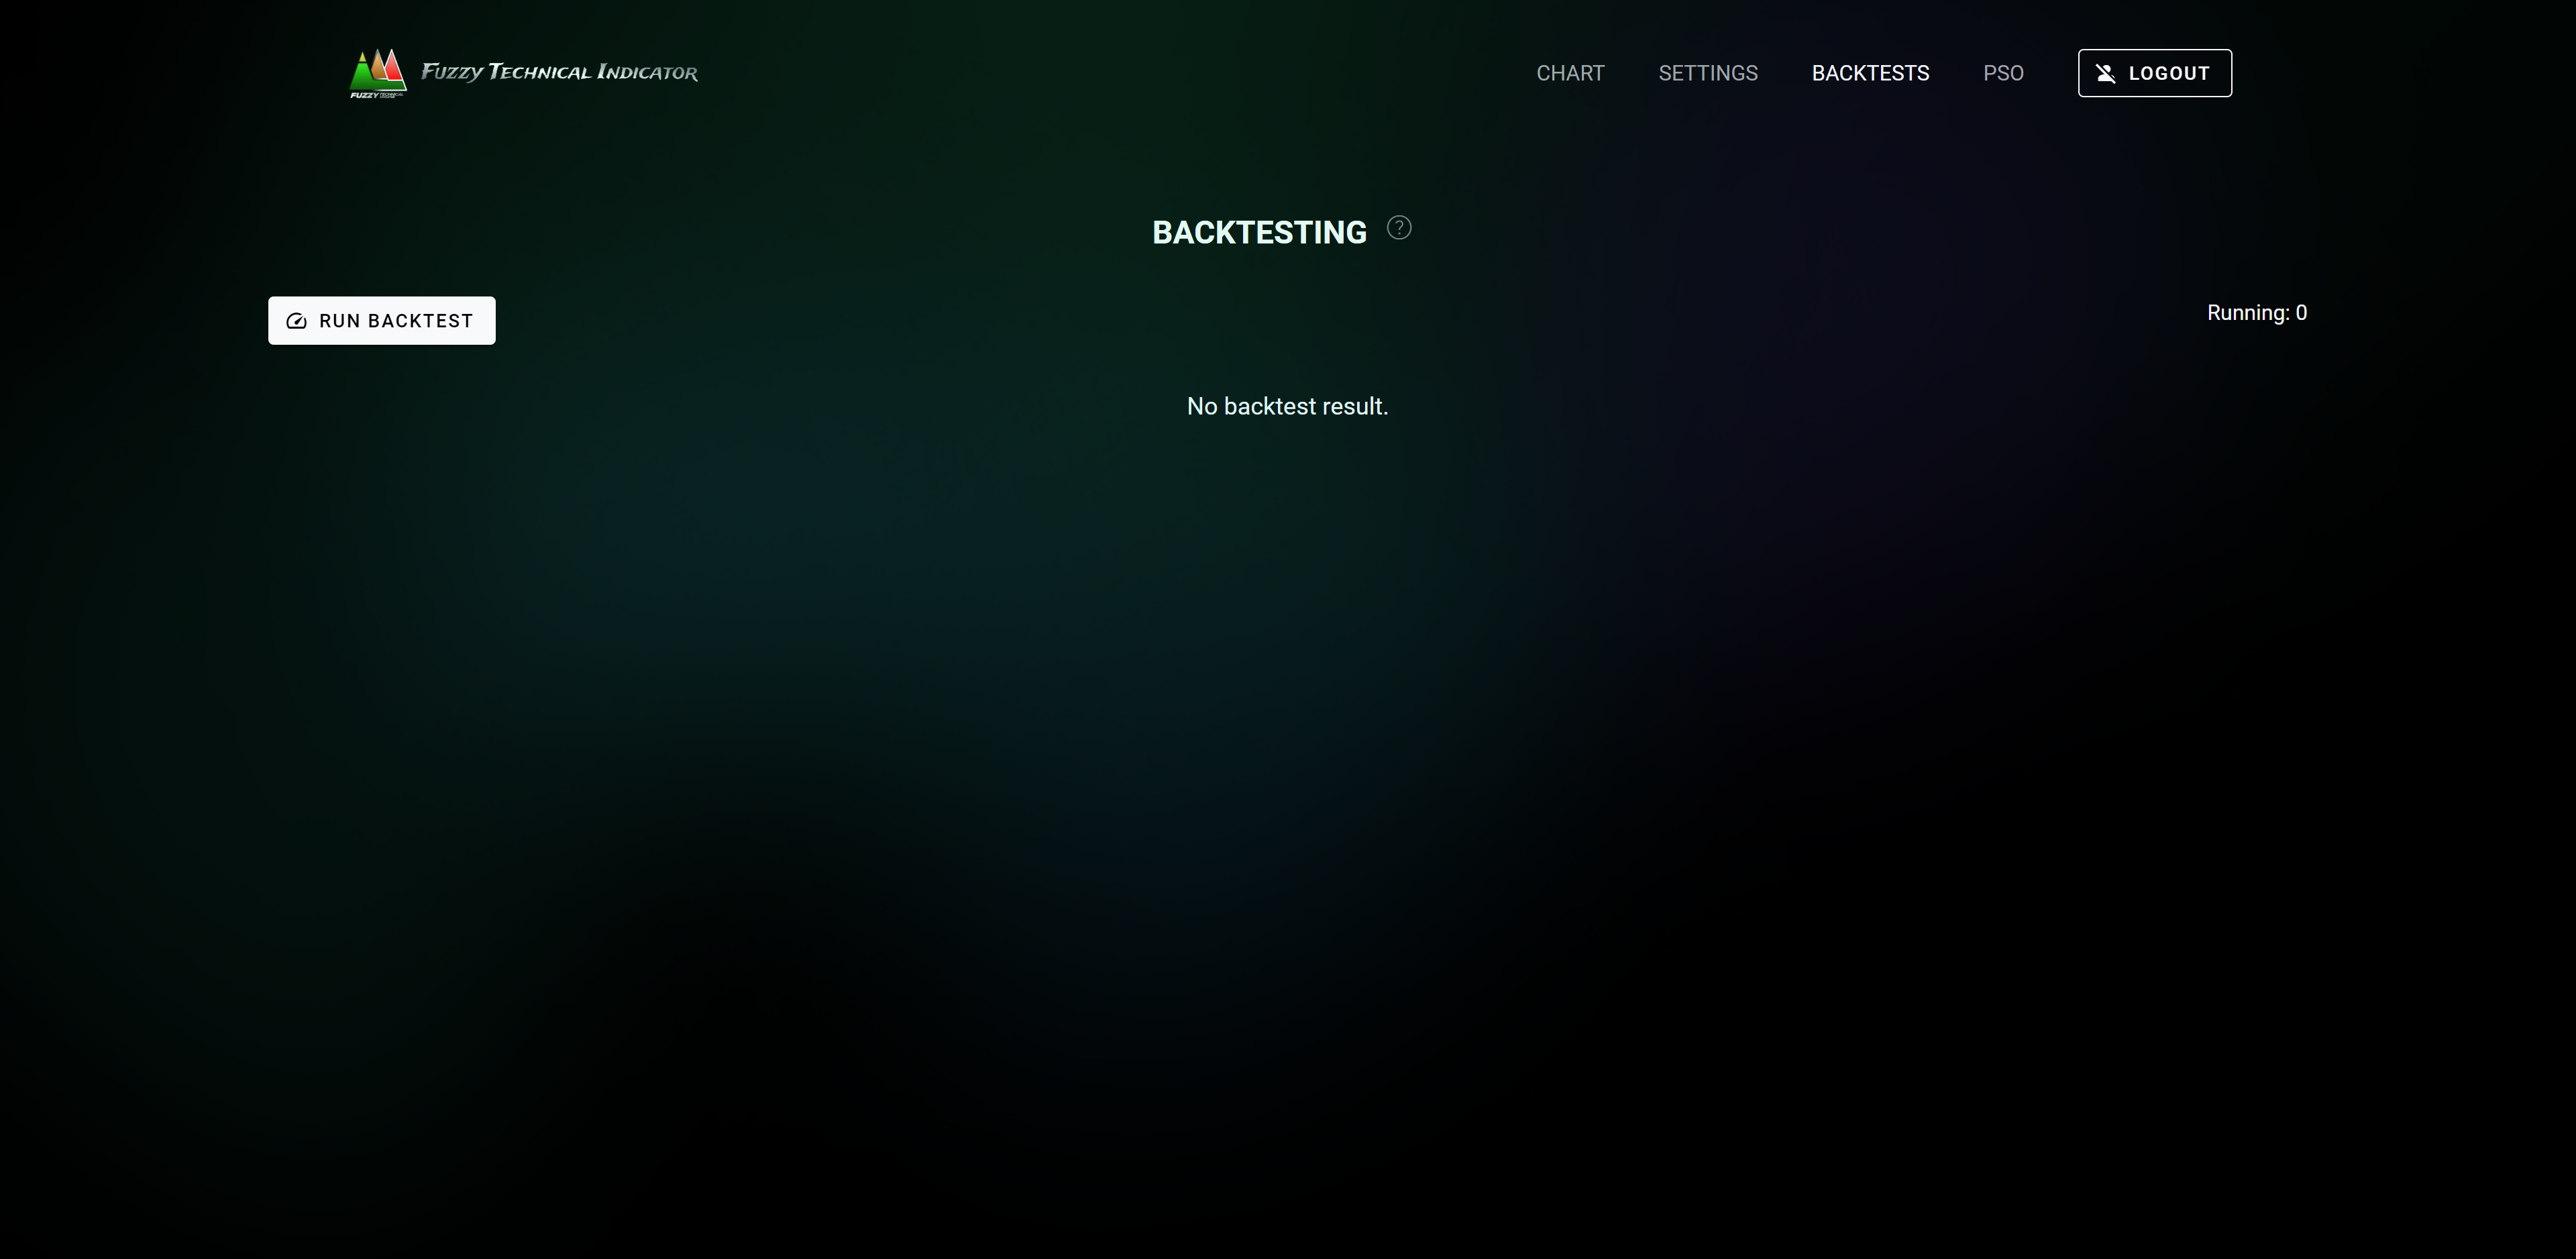
\includegraphics[width=\textwidth]{images/web-tuts/backtest-no-result.PNG}
    \caption{เว็บแอปพลิเคชัน หน้า Backtests (ยังไม่มีผลลัพธ์การทดสอบ)}
    \label{fig:backtest-no-result}
\end{figure}
\FloatBarrier
สามารถกดปุ่ม RUN BACKTEST เพื่อเข้าสู่หน้าการตั้งค่าการทดสอบ โดยเมื่อเข้ามาแล้วจะต้องมีการตั้งค่า 2 ส่วนคือ Trading Essentials และ Ordering Conditions
\begin{figure}[ht]
    \centering
    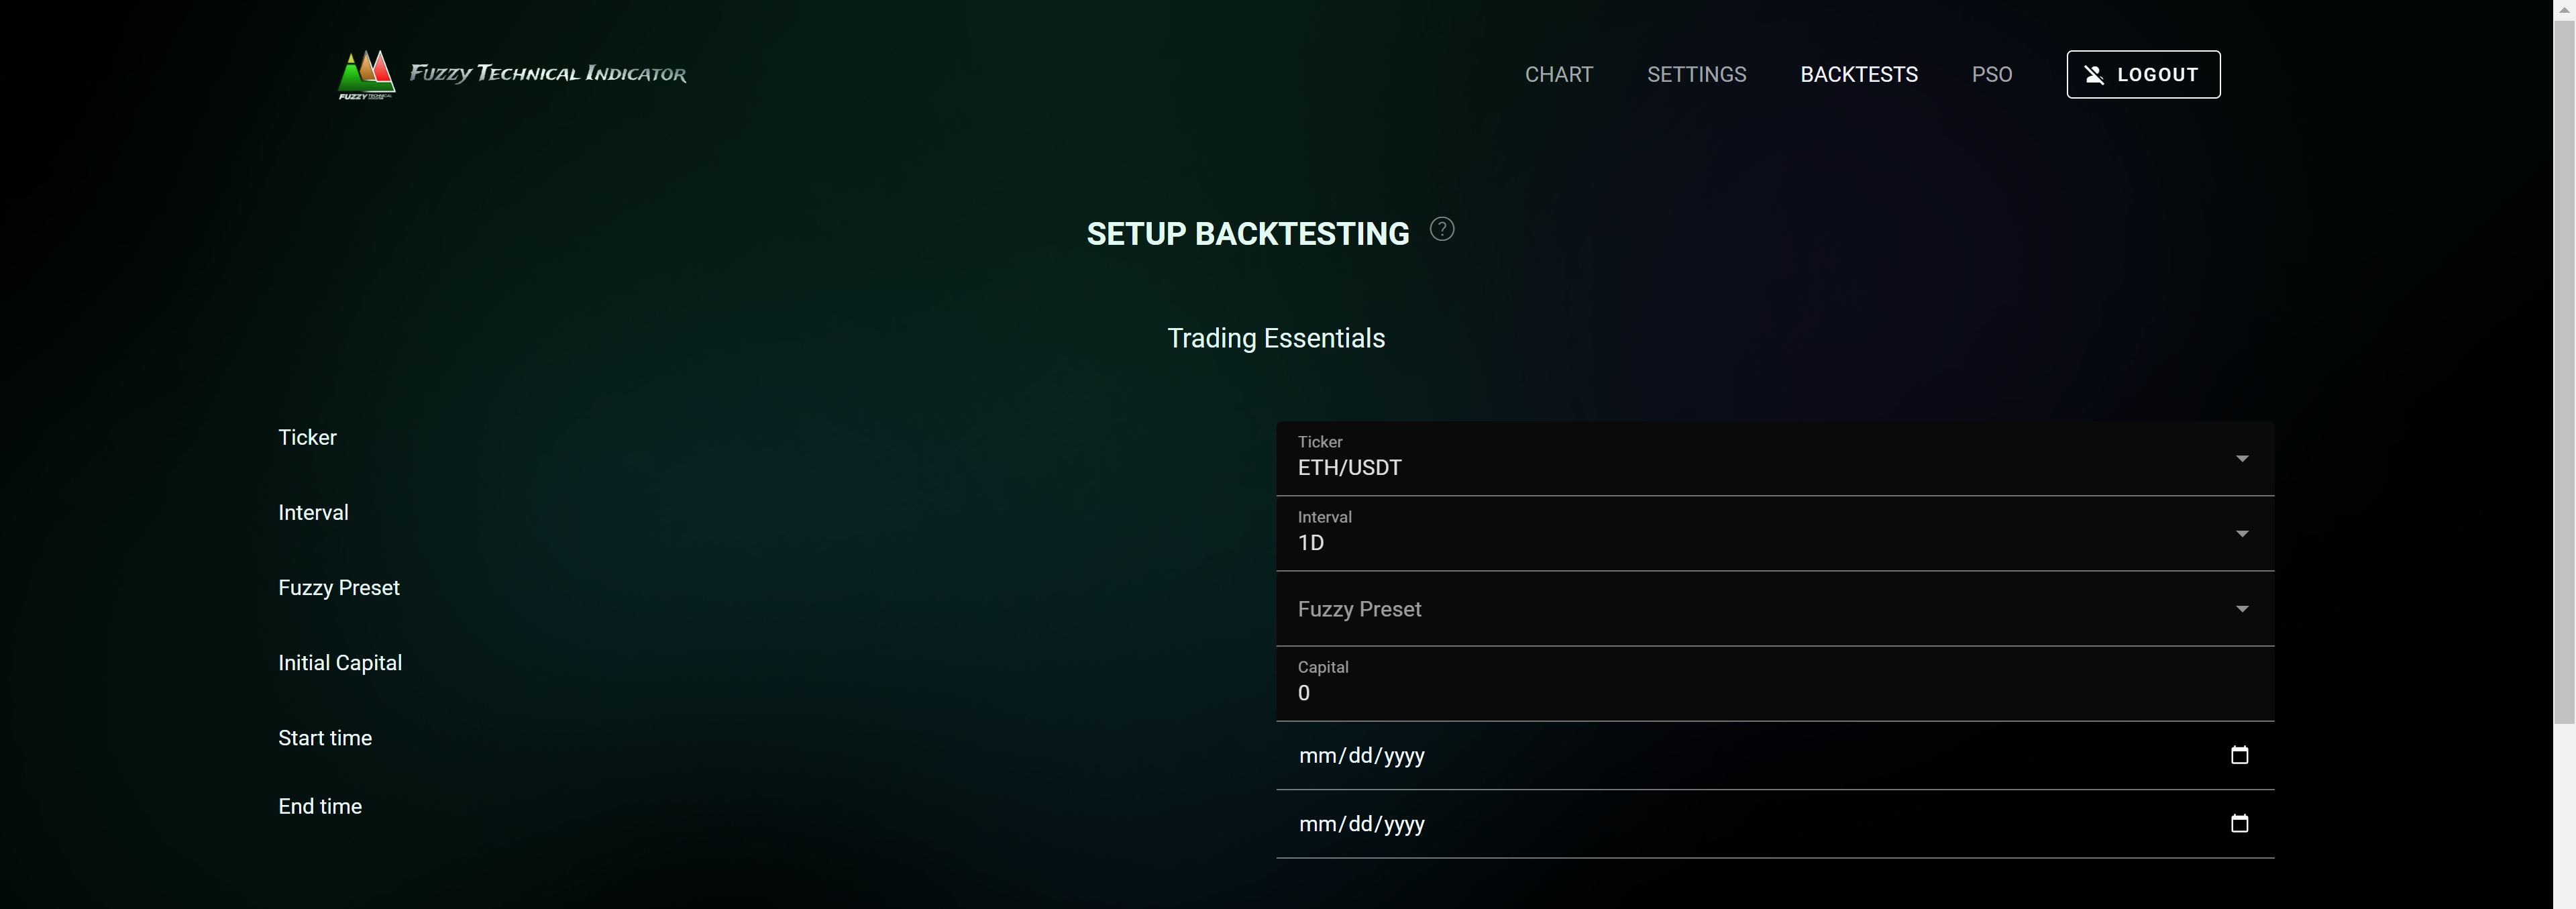
\includegraphics[width=\textwidth]{images/web-tuts/backtest-setup-trade-ess.PNG}
    \caption{Backtest การตั้งค่าการทดสอบในส่วน Trading Essentials}
    \label{fig:backtest-setup-trade-ess}
\end{figure}
\FloatBarrier
การตั้งค่า Trading Essentials จะประกอบไปด้วย
\begin{enumerate}
    \overfullrule=0pt
    \item Ticker สำหรับเลือกสินทรัพย์ในตลาดที่ต้องการทดสอบ
    \item Interval เลือก Timeframe ของสินทรัพย์ (1H, 4H, 1D)
    \item Fuzzy Preset เลือก Preset ที่เราสร้างไว้เพื่อใช้ในการทดสอบ
    \item Initial Capital กำหนดจำนวนเงินทุนตั้งต้น (USD)
    \item Start time วันที่เริ่มทดสอบ
    \item End time วันที่จบการทดสอบ
\end{enumerate}
\begin{figure}[ht]
    \centering
    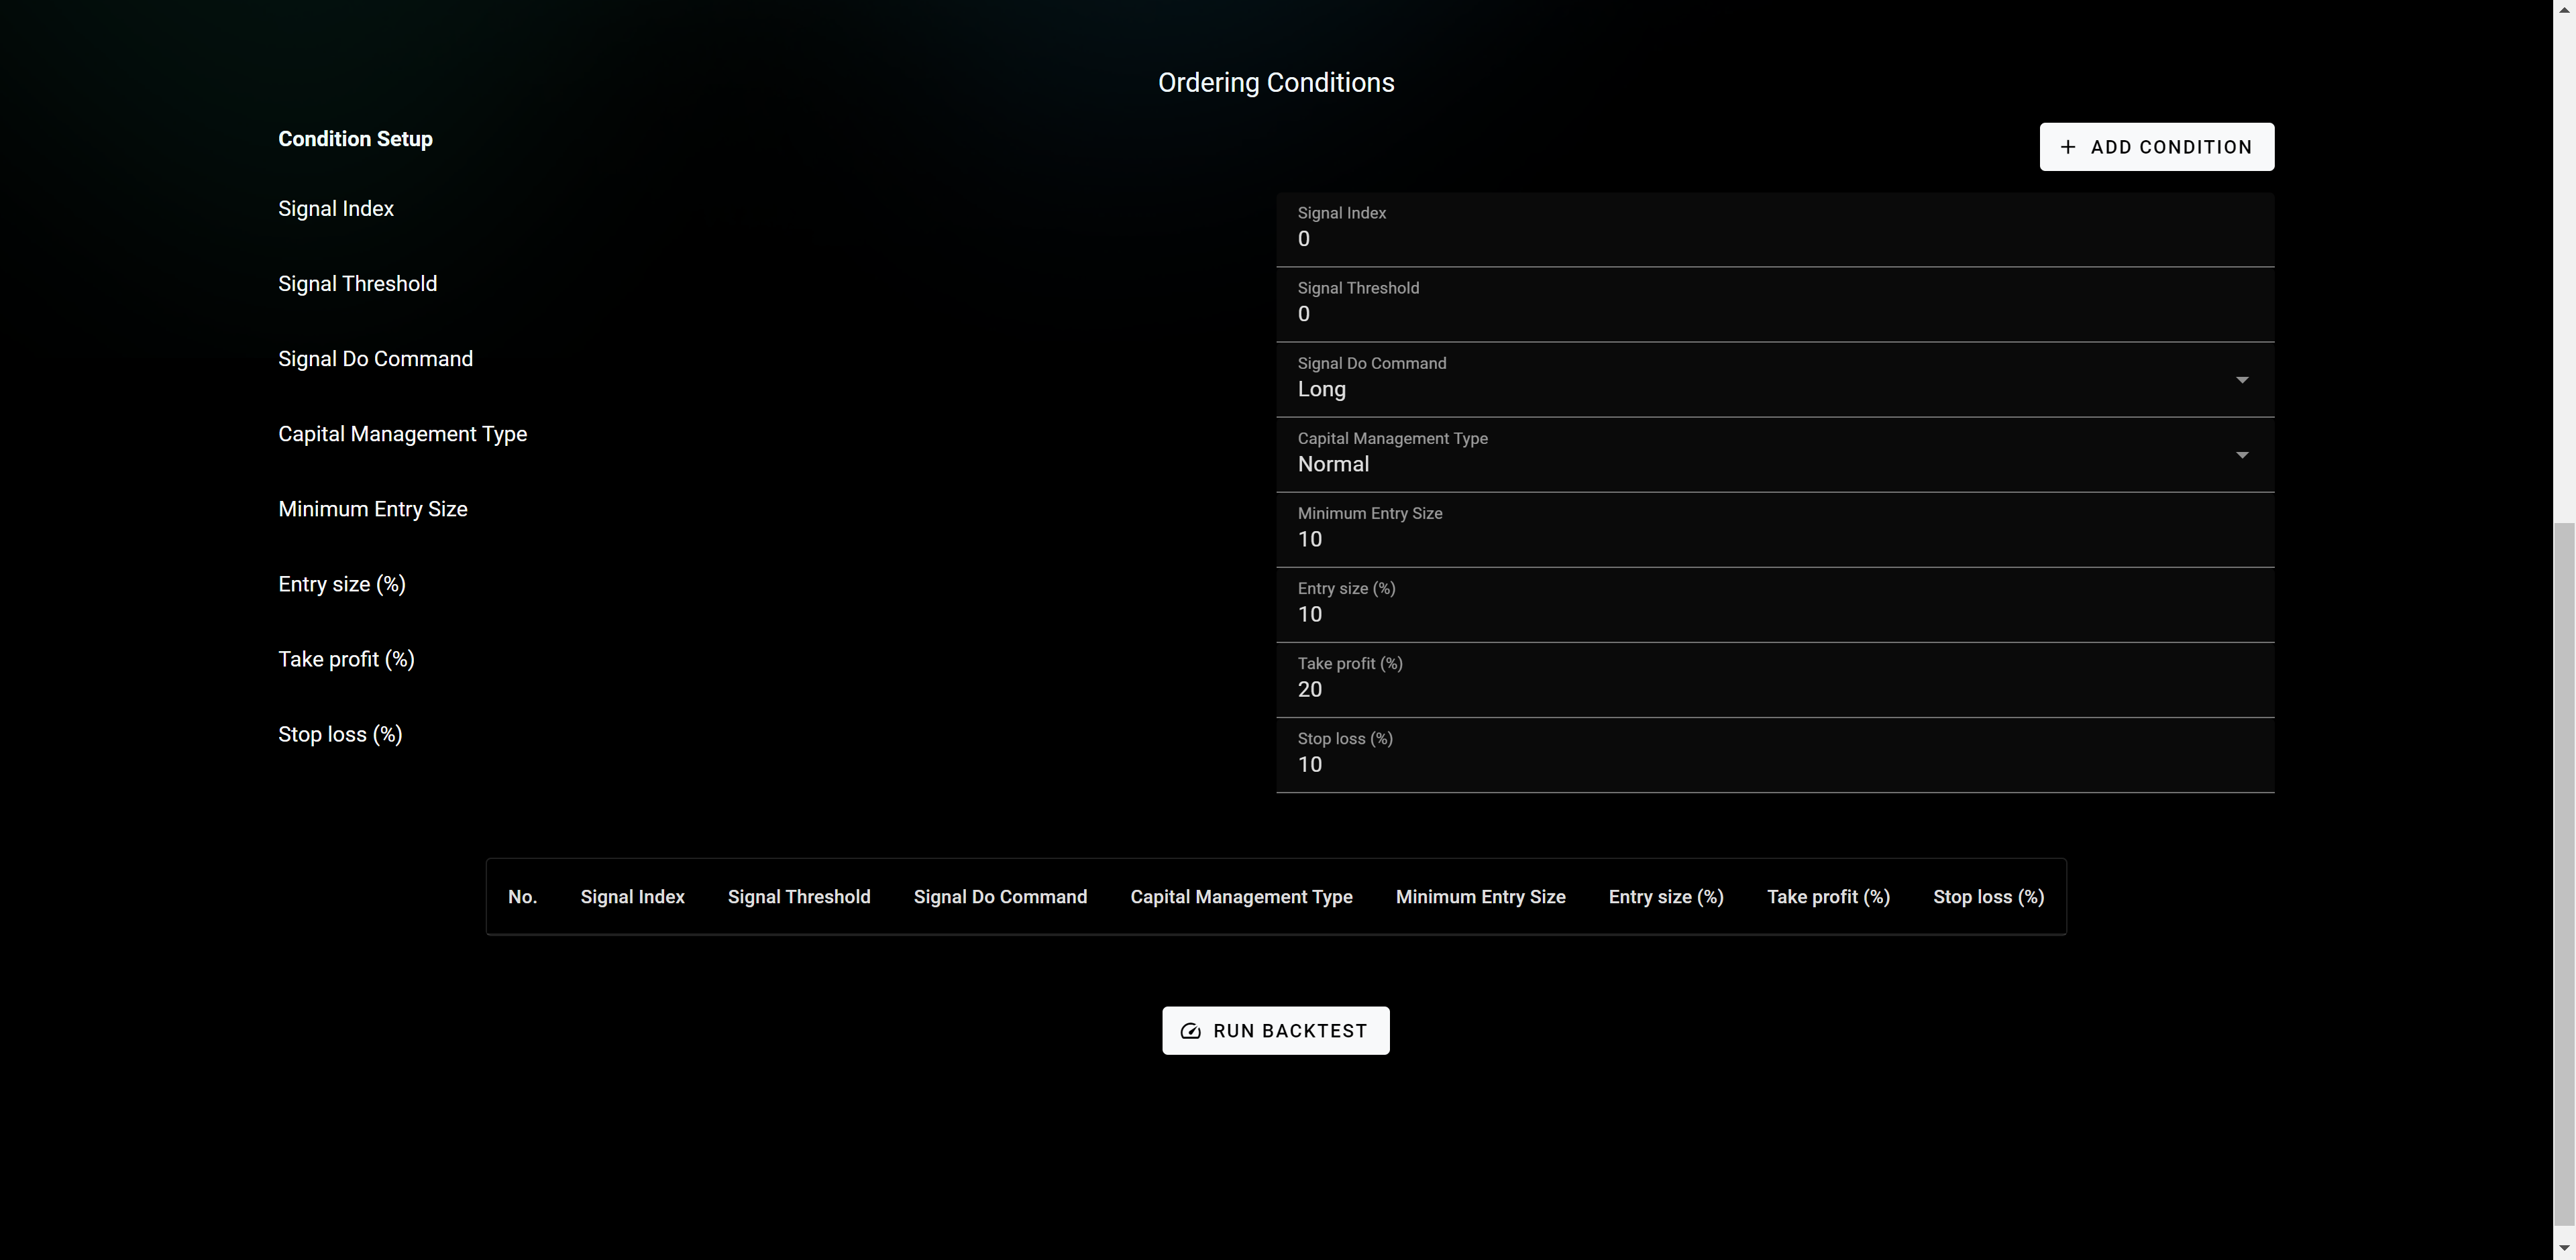
\includegraphics[width=\textwidth]{images/web-tuts/backtest-setup-order-conds.PNG}
    \caption{Backtest การตั้งค่าการทดสอบในส่วน Ordering Conditions}
    \label{fig:backtest-setup-order-conds}
\end{figure}
\FloatBarrier
การตั้งค่า Ordering Conditions เพือกำหนดเงื่อนไขการ Entry และ Exit Order จะประกอบไปด้วย
\begin{enumerate}
    \overfullrule=0pt
    \item Signal Index เลขดัชนีสัญญาณ Fuzzy
    \item Signal Threshold ระดับในการสั่งการสัญญาณ
    \item Signal Do Command คำสั่งที่จะทำเมื่อสัญญาณถึงระดับ Threshold
    \item Capital Management Type รูปแบบการจัดการเงินทุน (Normal, Liquid-F)
    \item Minimum Entry Size จำนวนเงินในการ Entry ต่ำสุด (USD)
    \item Entry Size ขนาด Entry จากจำนวนเงินต้นทุน
    \item Take Profit ขนาด Profit จากจุดที่ ซื้อ/ขาย เพื่อทำการปิด Order
    \item Stop Loss ขนาด Loss จากจุดที่ ซื้อ/ขาย เพื่อทำการปิด Order
\end{enumerate}
โดยจะสามารถเพิ่ม Conditions ได้หลายเงื่อนไขโดยเมื่อตั้งค่าดังกล่าวแล้วให้ทำการกดปุ่ม ADD CONDITION เงื่อนไขทั้งหมดที่ตั้งค่าจะแสดงในตารางดังรูป \ref{fig:backtest-setup-conditioned} จากนั้นทำการกดปุ่ม RUN BACKTEST เพื่อเริ่มการทดสอบ
\begin{figure}[ht]
    \centering
    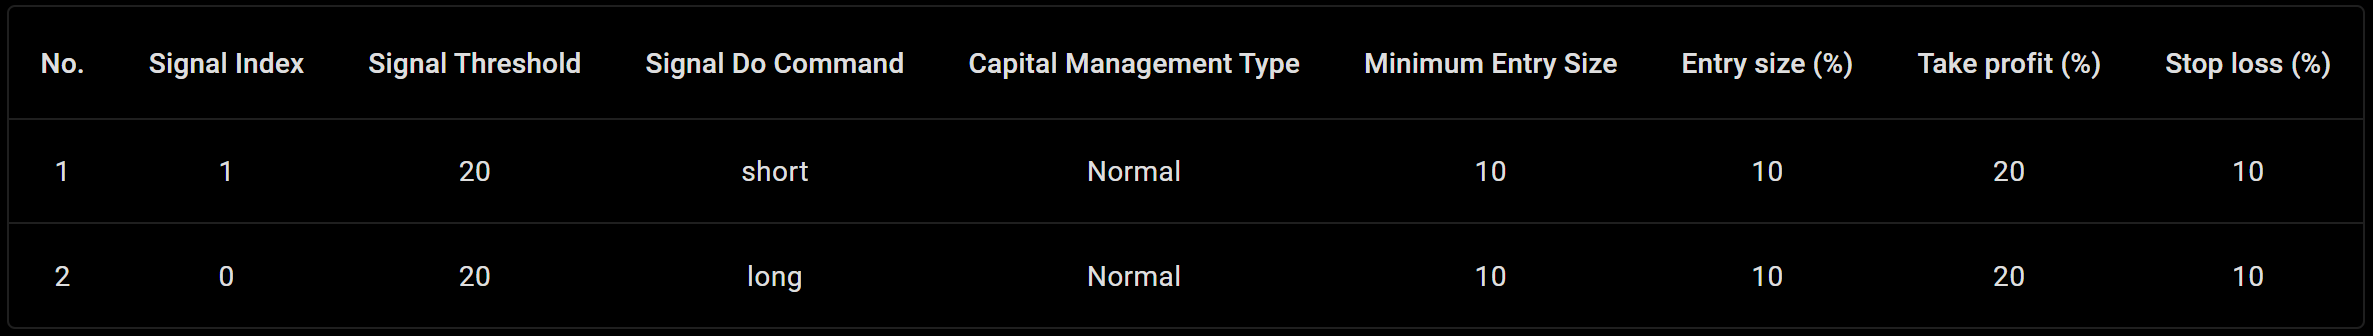
\includegraphics[width=\textwidth]{images/web-tuts/backtest-setup-conditioned.PNG}
    \caption{ตารางแสดง Ordering Conditions}
    \label{fig:backtest-setup-conditioned}
\end{figure}
\FloatBarrier
เมื่อทำการกดเริ่มการทดสอบแล้วจะกลับมาหน้าแสดงผลลัพธ์การทดสอบโดยจะมีสถานะการทดสอบแสดงดังรูป \ref{fig:backtest-running} ว่าขณะนี้มีการดำเนินการทดสอบอยู่กี่ตัว โดยเมื่อเสร็จสิ้นแล้วจะแสดงกราฟการปรับเปลี่ยนของจำนวนเงินทุนและข้อมูลอย่าง จำนวนการ Trades, ผลกำไร/ขาดทุน และอื่นๆ ดังรูป \ref{fig:backtest-with-result}
\begin{figure}[ht]
    \centering
    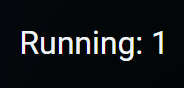
\includegraphics[scale=0.75]{images/web-tuts/backtest-running.PNG}
    \caption{สถานะแสดงจำนวนการทดสอบ Backtest ที่กำลังดำเนินการ}
    \label{fig:backtest-running}
\end{figure}
\begin{figure}[ht]
    \centering
    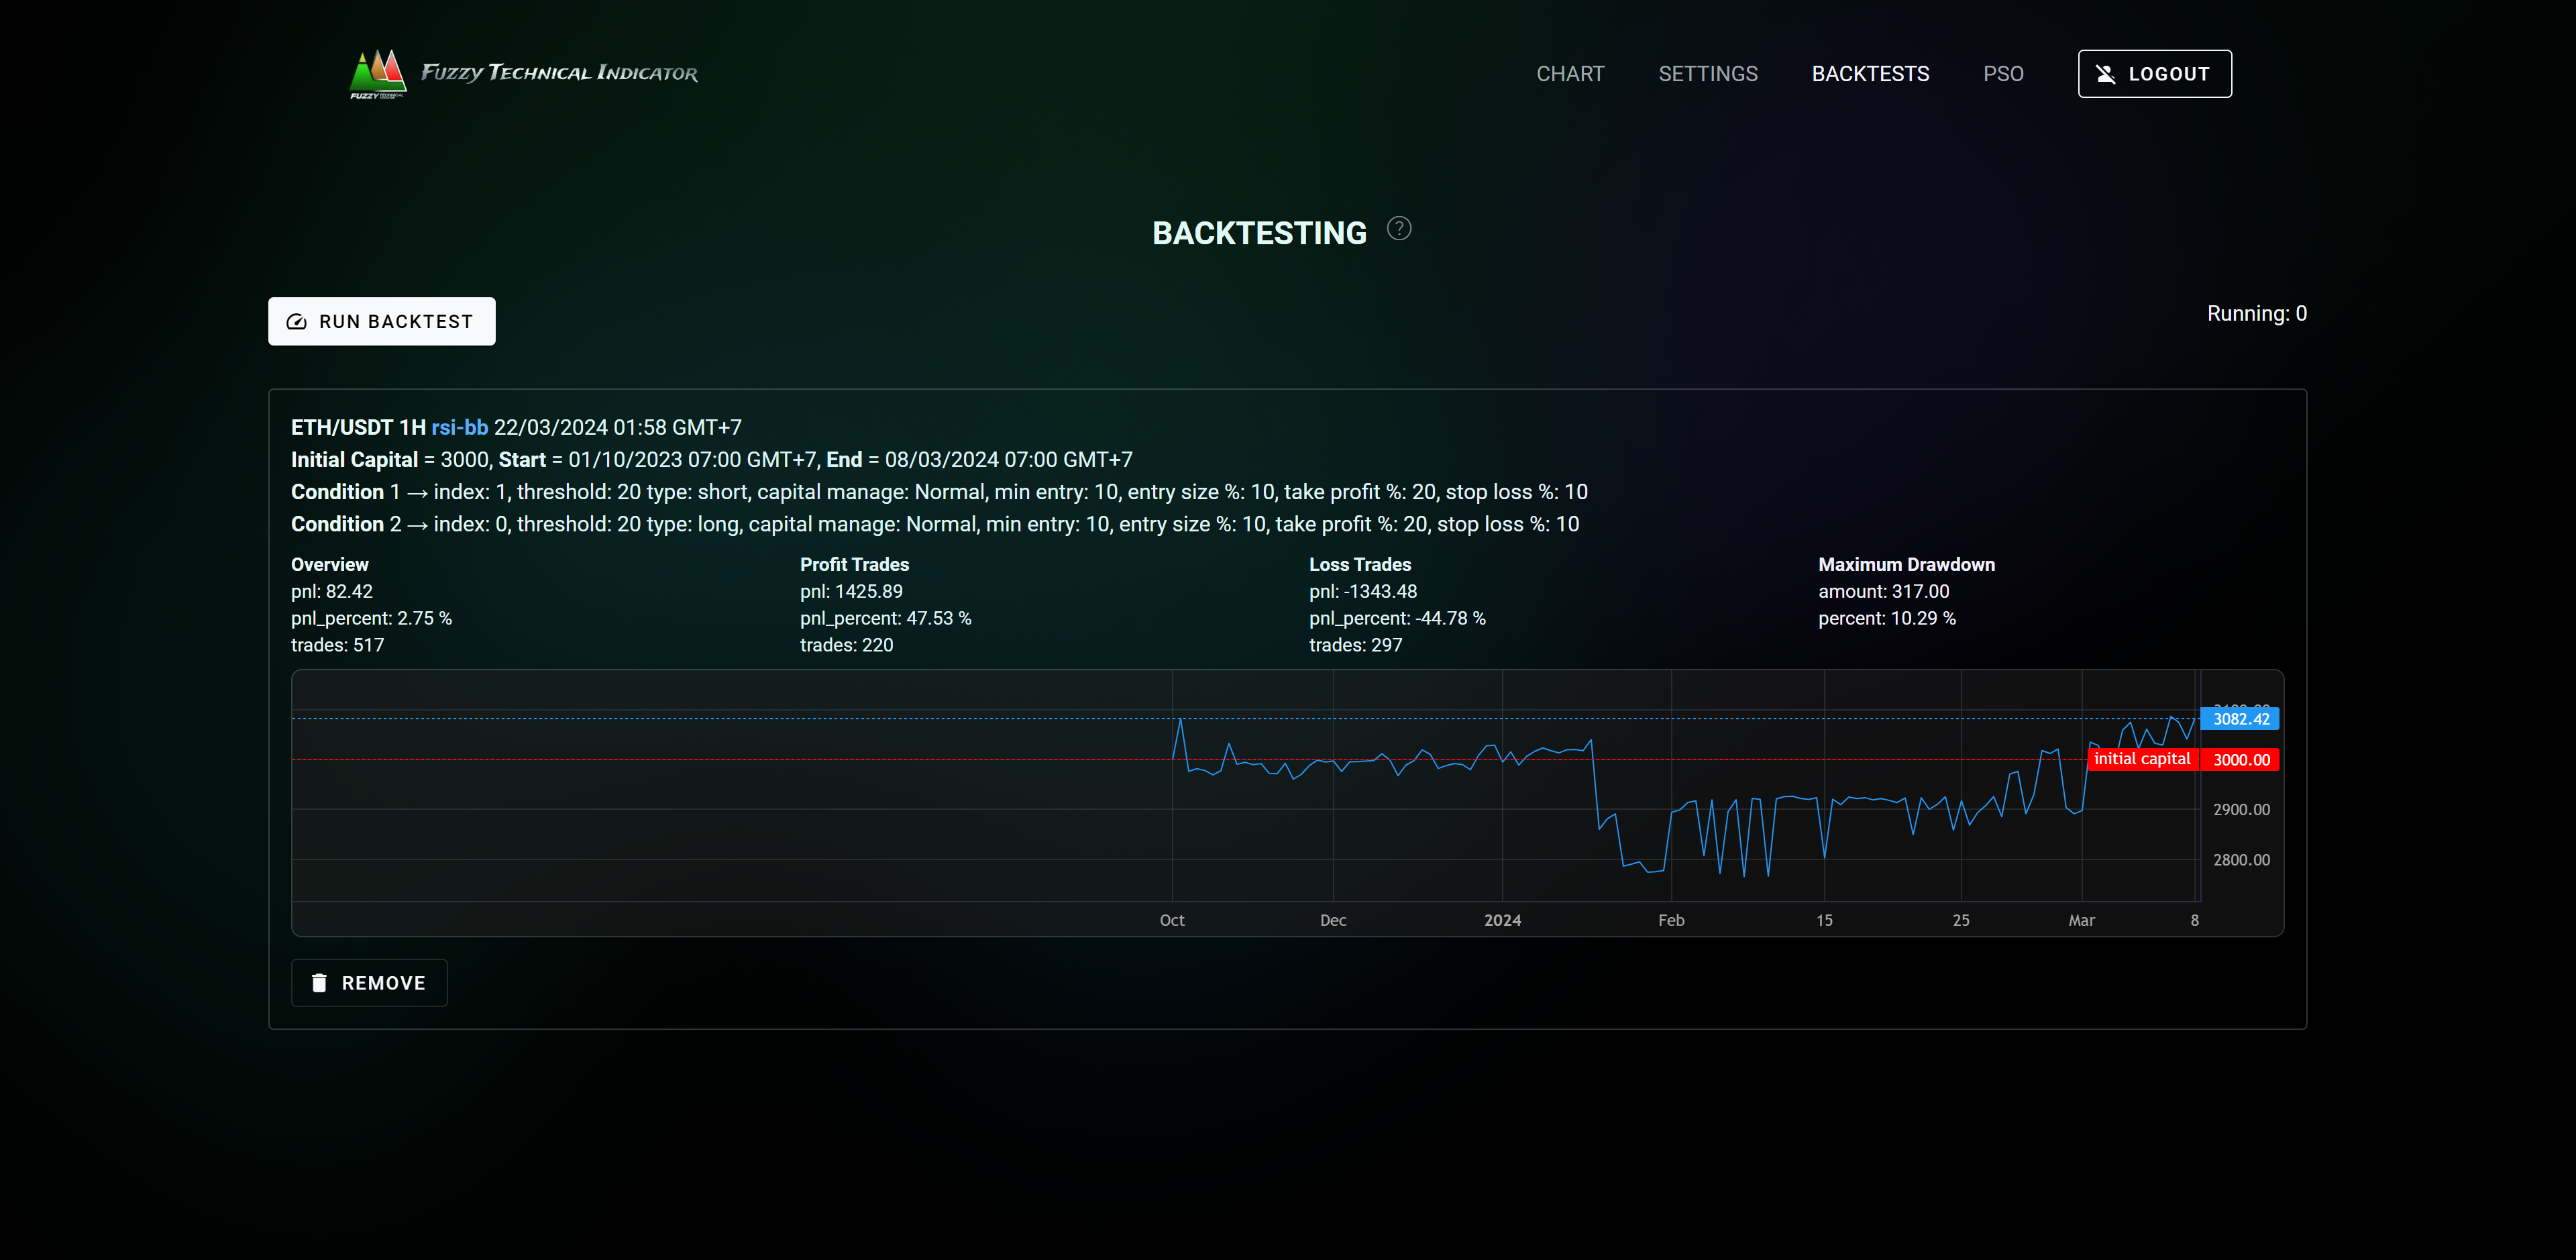
\includegraphics[width=\textwidth]{images/web-tuts/backtest-with-result.PNG}
    \caption{กราฟแสดงผลลัพธ์การทดสอบ Backtest}
    \label{fig:backtest-with-result}
\end{figure}
\FloatBarrier

\subsubsection{การใช้งานหน้า PSO}
หน้า PSO สำหรับการปรับจูนตัวแปรทางภาษาใน Fuzzy Preset ด้วย PSO โดยการใช้งานจะคล้ายกับหน้า Backtest แต่จะมีส่วนที่จะต้องตั้งค่าเพิ่มคือ PSO Parameters ทำการเข้าสู่หน้าตั้งค่าโดยกดที่ปุ่ม RUN PSO
\begin{figure}[ht]
    \centering
    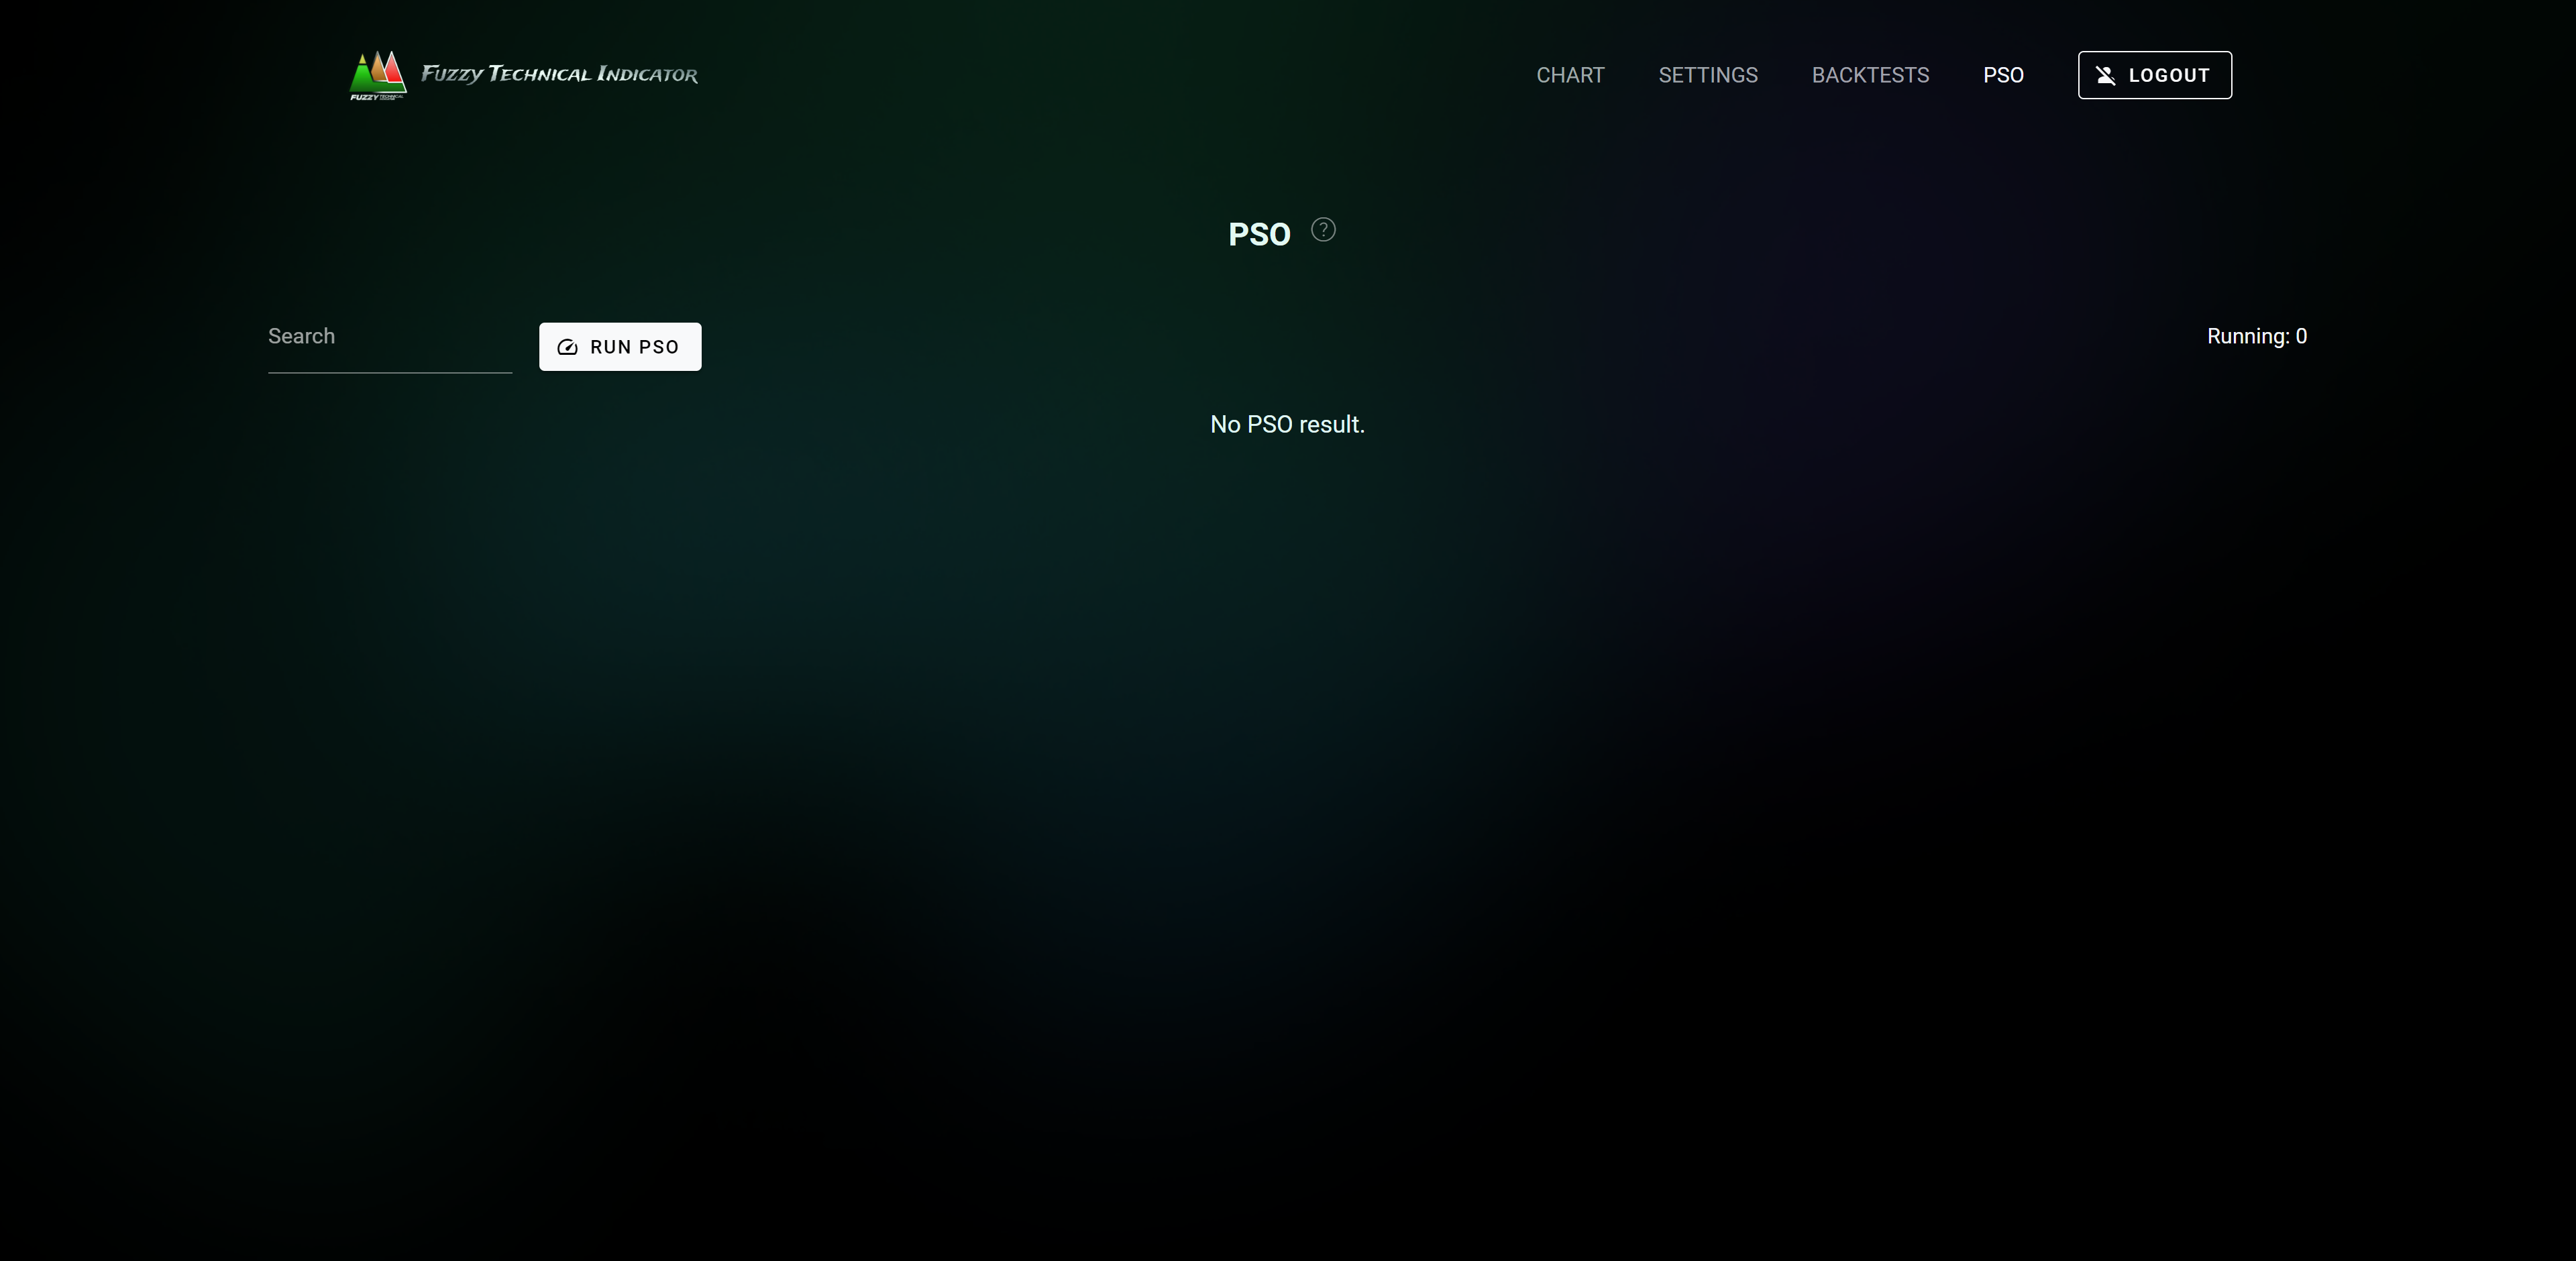
\includegraphics[width=\textwidth]{images/web-tuts/pso-no-result.PNG}
    \caption{เว็บแอปพลิเคชัน หน้า PSO (ยังไม่มีผลลัพธ์)}
    \label{fig:pso-no-result}
\end{figure}
\FloatBarrier
\begin{figure}[ht]
    \centering
    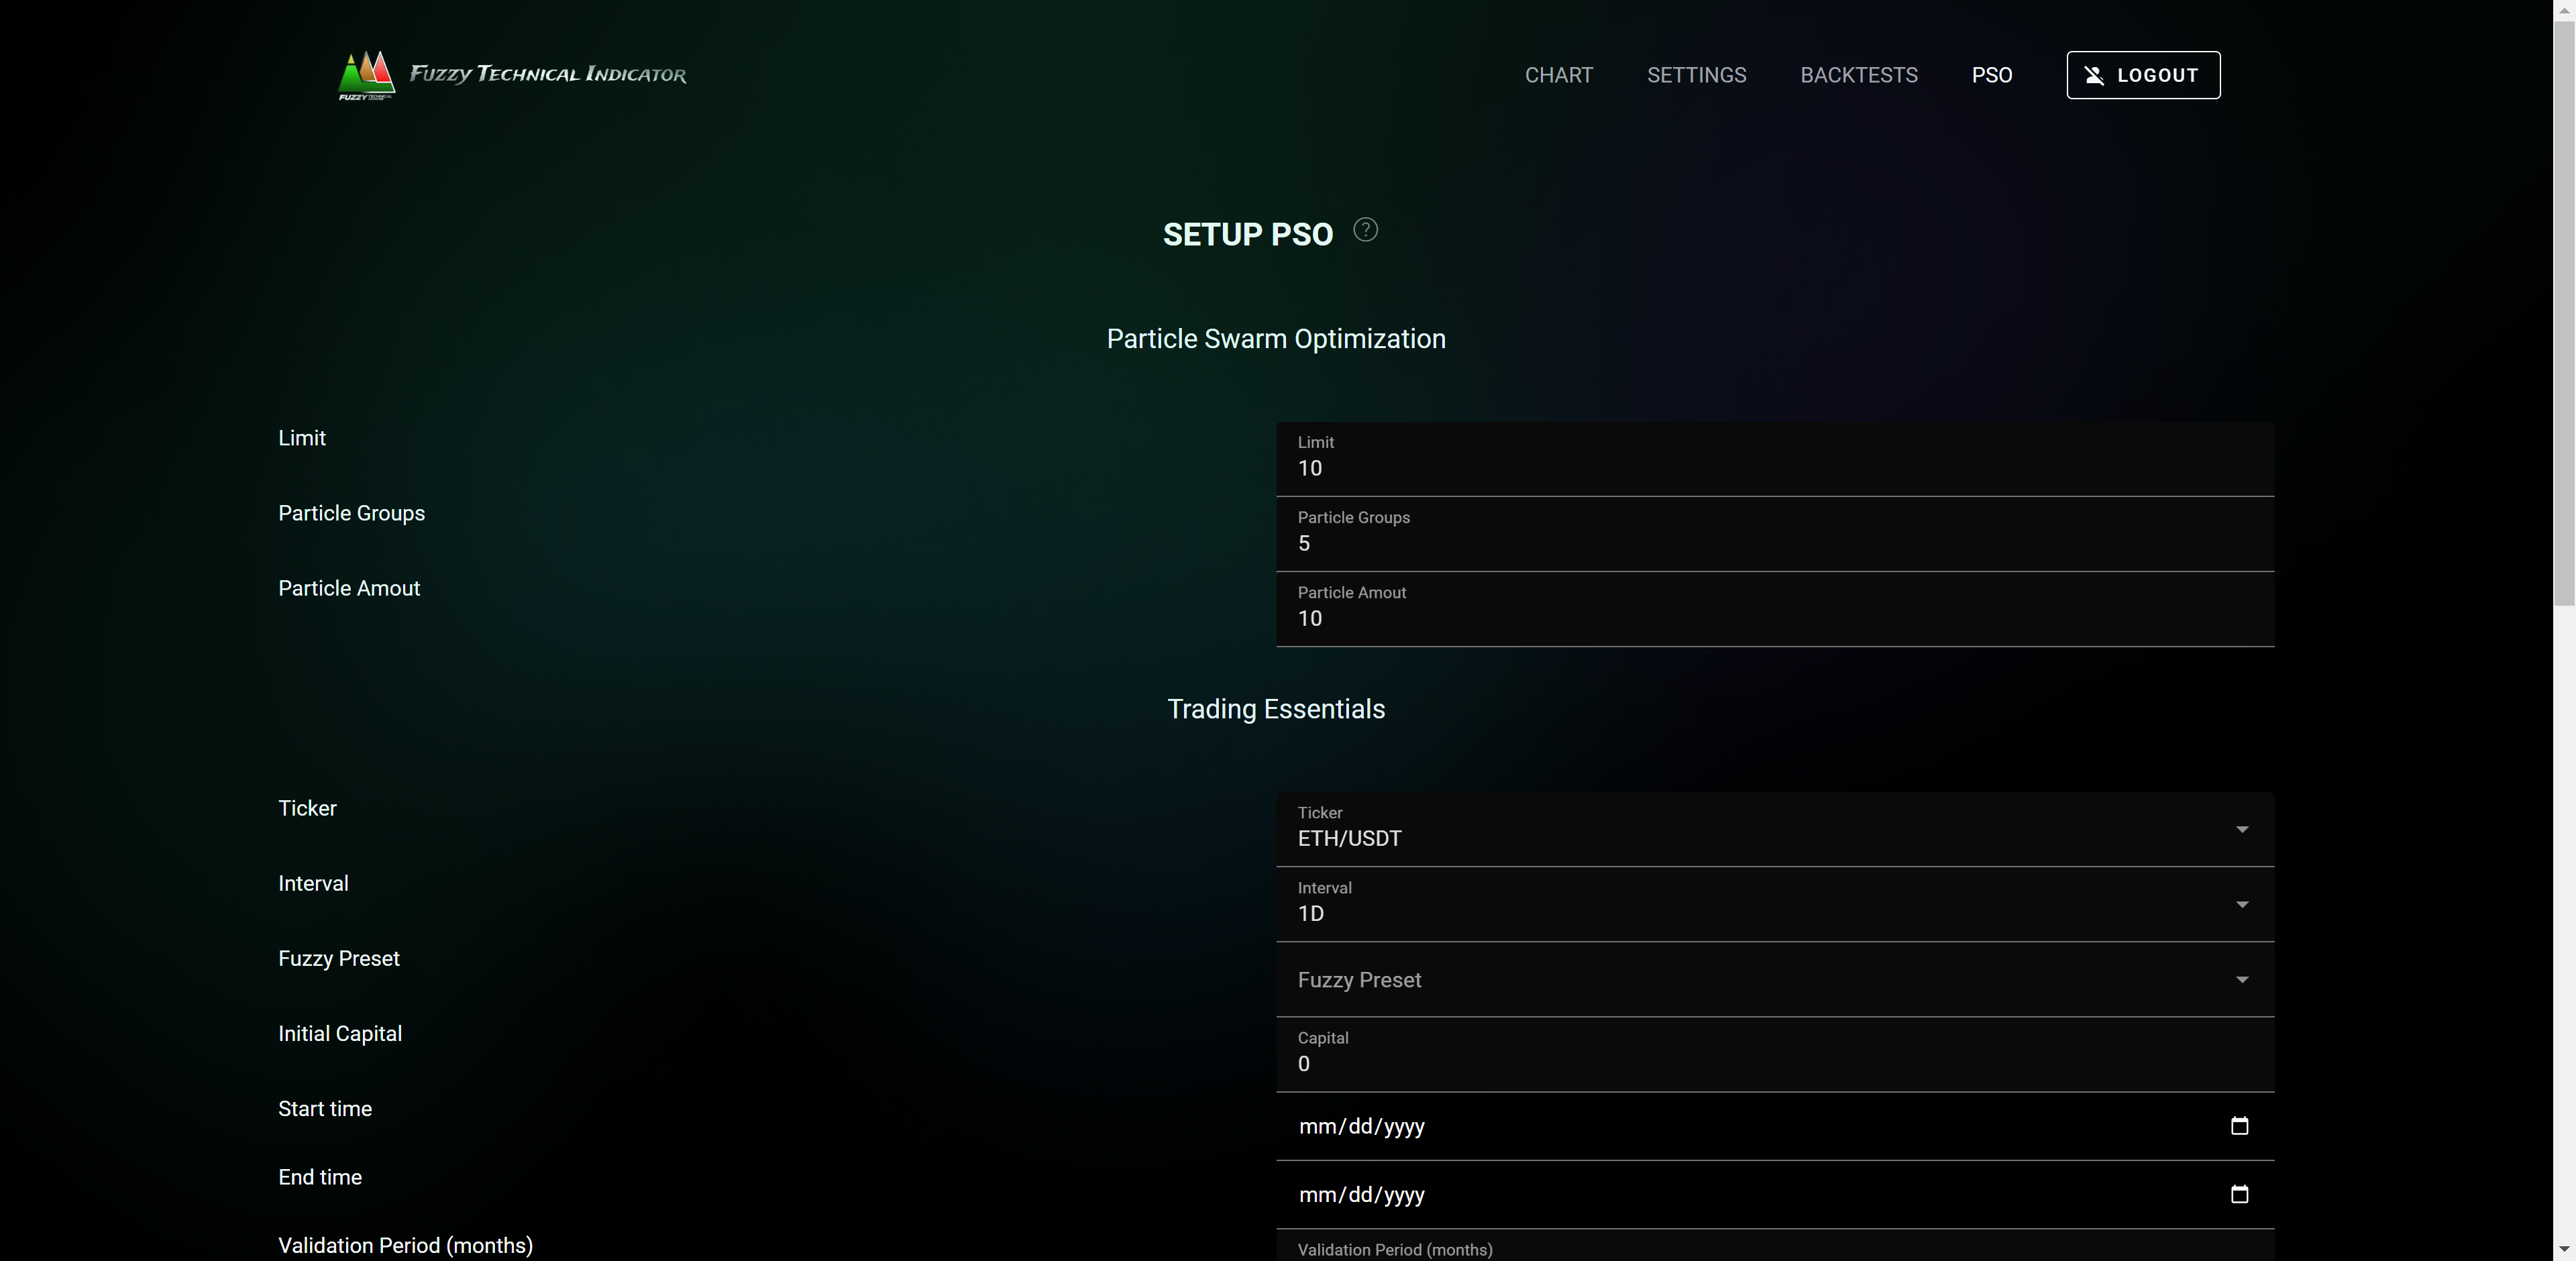
\includegraphics[width=\textwidth]{images/web-tuts/pso-setup-params.PNG}
    \caption{การตั้งค่า PSO Parameters}
    \label{fig:pso-setup-params}
\end{figure}
\FloatBarrier
การตั้งค่า Parameters ของ PSO จะประกอบไปด้วย
\begin{enumerate}
    \overfullrule=0pt
    \item Limit จำนวน Iteration ที่จะหยุด
    \item Particle Groups จำนวนกลุ่มของอนุภาค
    \item Particle Amount จำนวนอนุภาคในกลุ่ม
\end{enumerate}
และในส่วนของ Trading Essentials จะเหมือนกันกับ Backtest แต่จะมีการตั้ง Validation Period (months) เพิ่มเข้ามา คือระยะเวลาการทำ Validation เป็นจำนวนกี่เดือนก่อนหน้าช่วงเวลาการทดสอบ (ก่อน Start time) เมื่อทำการตั้งค่าเสร็จสิ้นกดปุ่ม RUN PSO เพื่อดำเนินการ
\begin{figure}[ht]
    \centering
    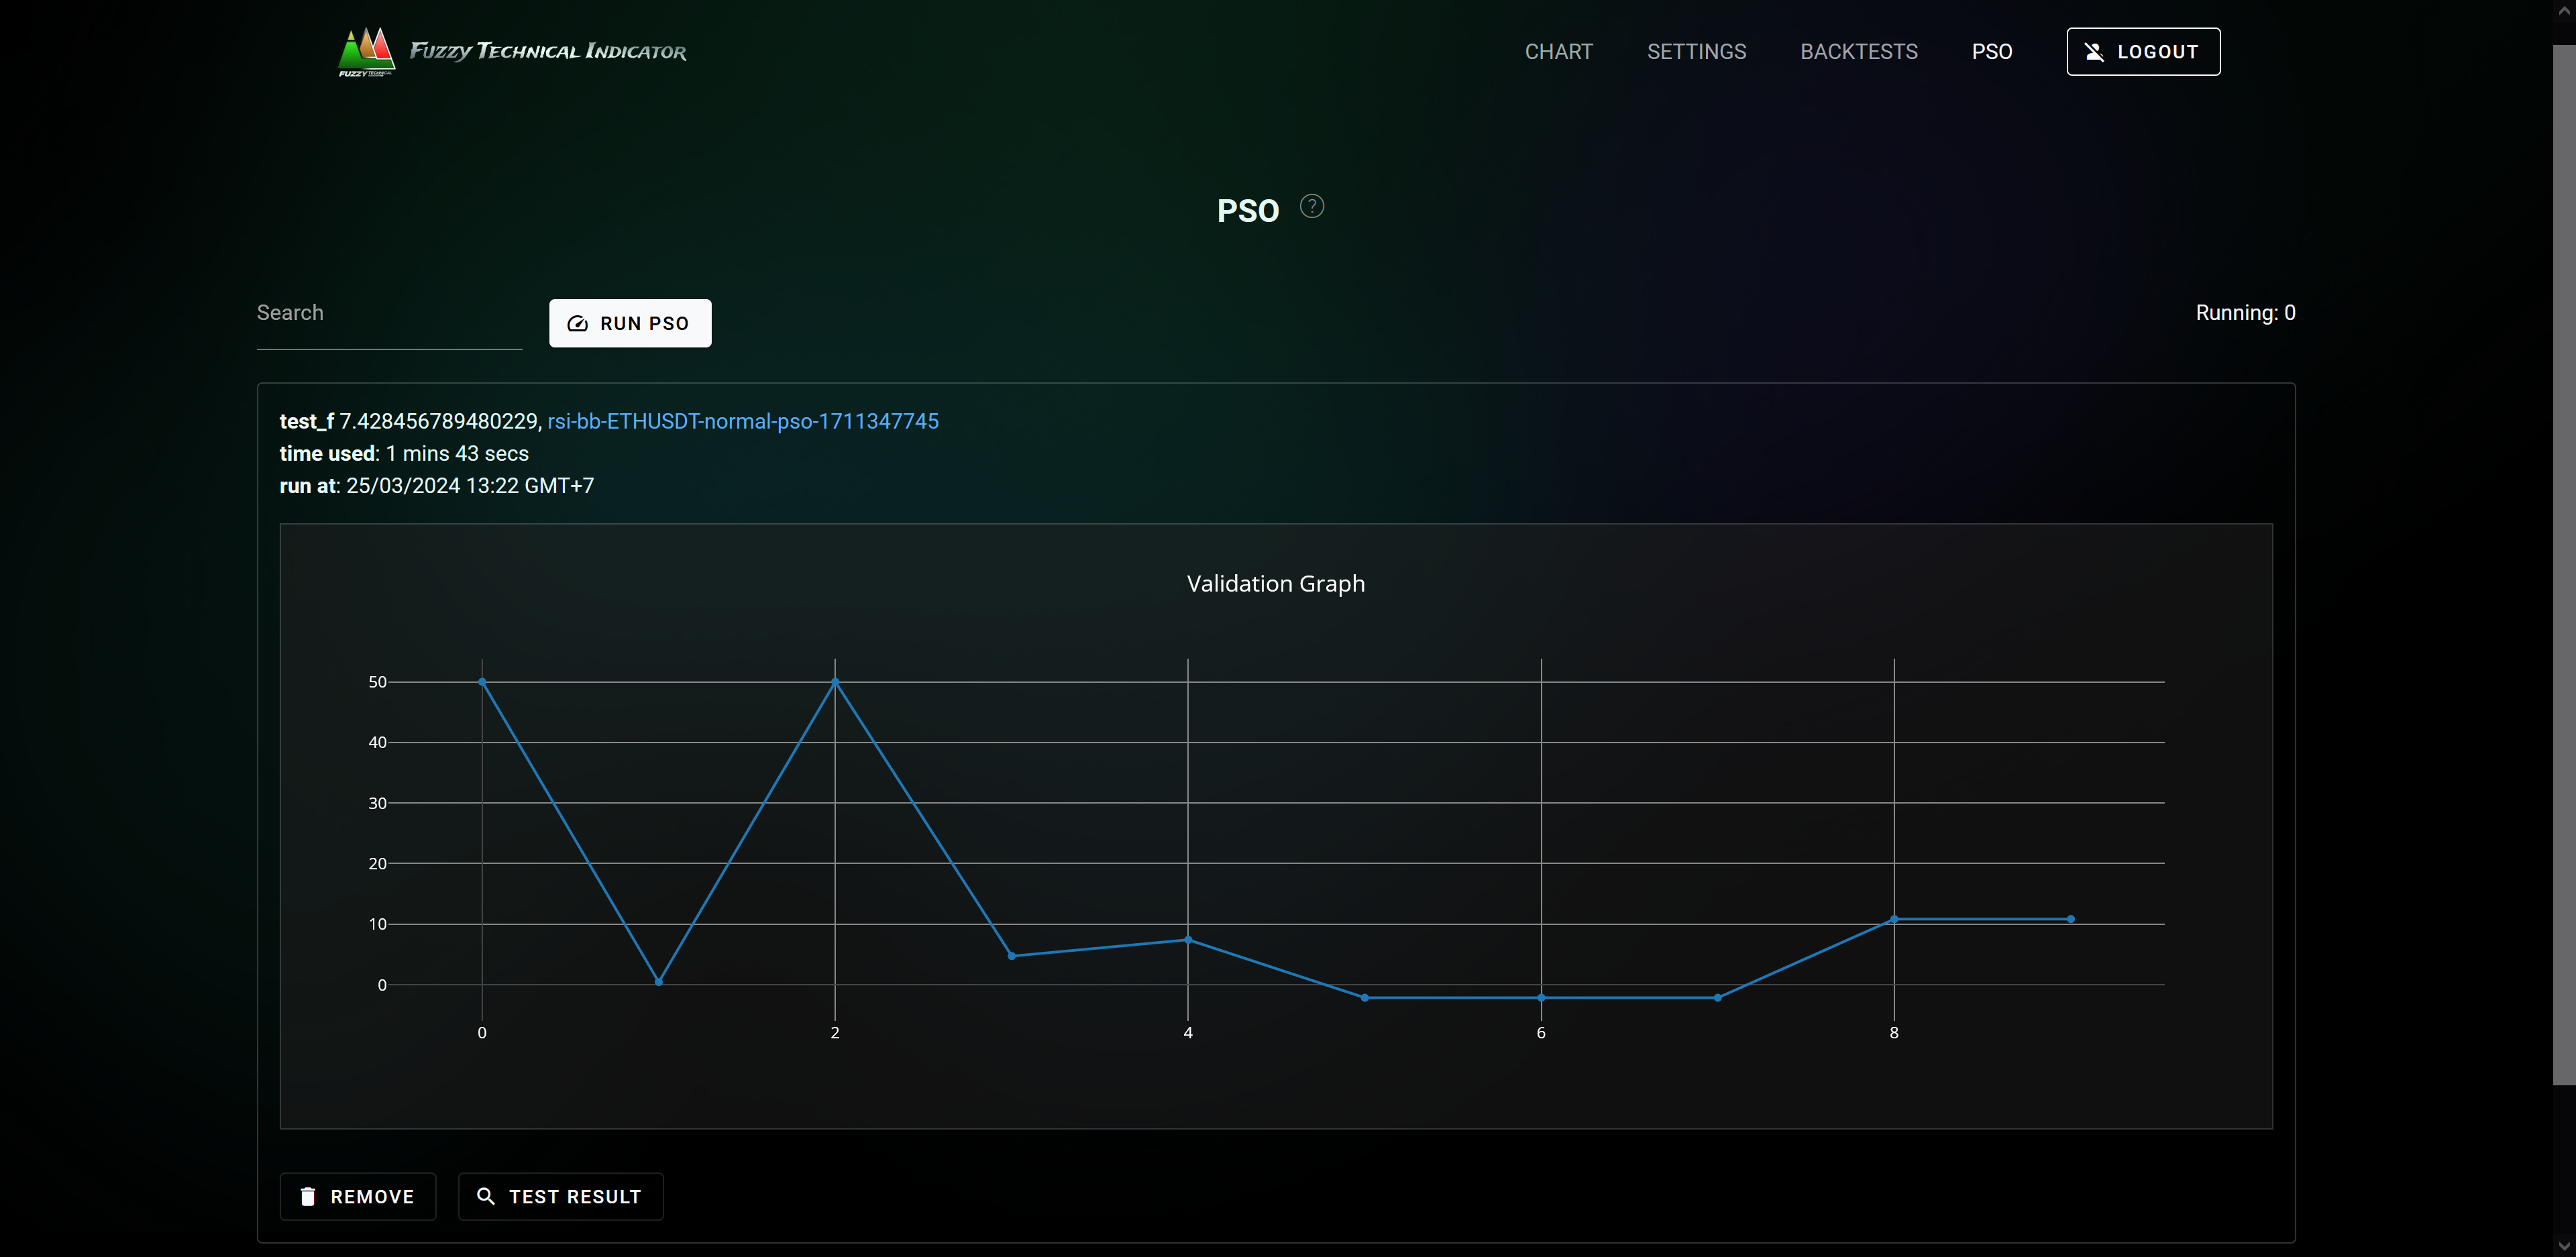
\includegraphics[width=\textwidth]{images/web-tuts/pso-result.PNG}
    \caption{กราฟแสดงผลลัพธ์การปรับจูน PSO (Validation Graph)}
    \label{fig:pso-result}
\end{figure}
\FloatBarrier
เมื่อทำการดำเนินการเสร็จจะแสดงผลลัพธ์ของการปรับจูนด้วย PSO ดังรูป \ref{fig:pso-result} และสามารถกดปุ่ม TEST RESULT เพื่อดูผลลัพธ์การทดสอบ Backtest บน Preset ที่ถูกปรับจูนตัวแปรทางภาษา PSO และ Validation ได้ดีที่สุด ดังรูป \ref{fig:pso-test-result}
\begin{figure}[ht]
    \centering
    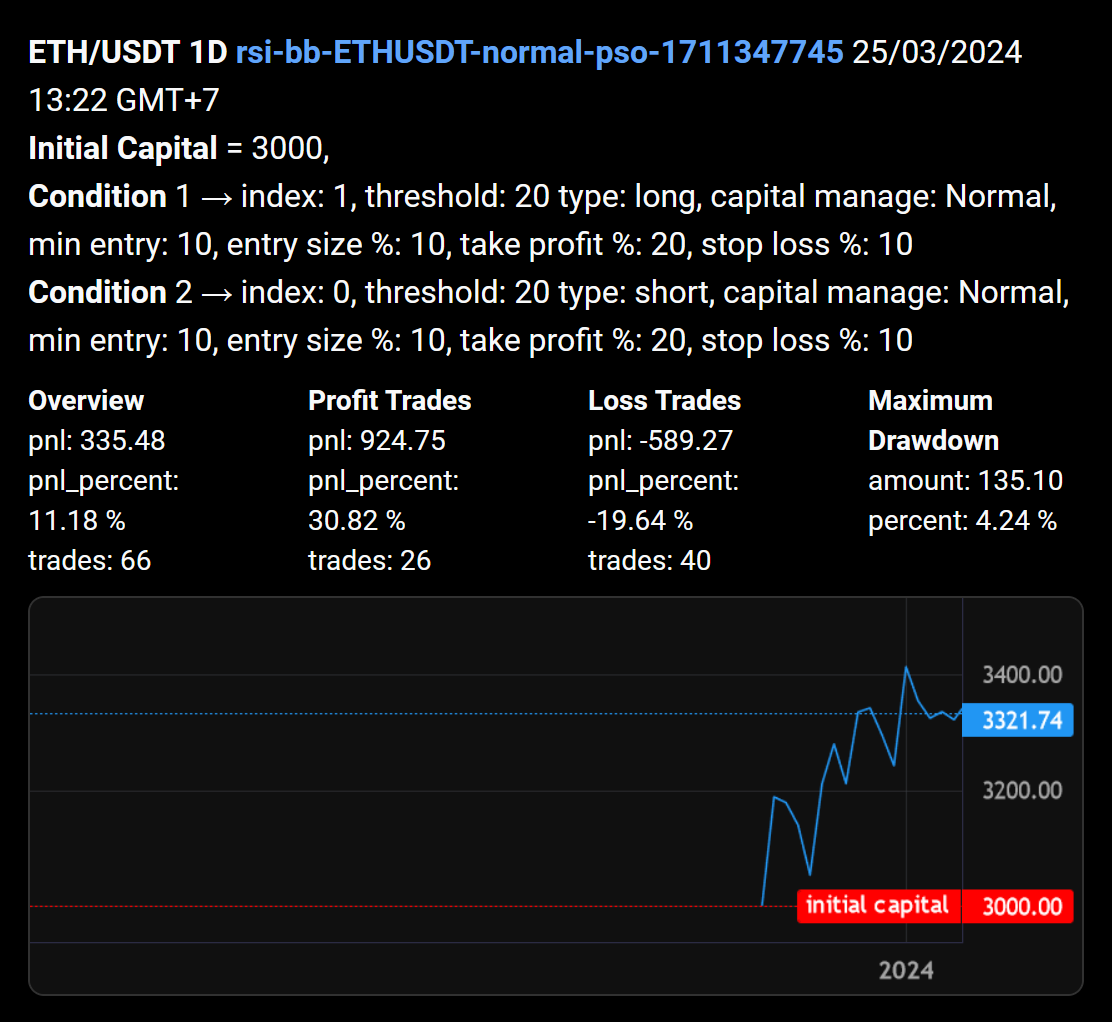
\includegraphics[scale=0.5]{images/web-tuts/pso-test-result.PNG}
    \caption{ผลการทดสอบ Backtest บน Preset ที่ถูกปรับจูนด้วย PSO และ Validation ได้ดีที่สุด}
    \label{fig:pso-test-result}
\end{figure}
\FloatBarrier
สามารถกดที่ชื่อ Preset (ตัวหนังสือสีฟ้า) คือ Preset ที่ถูกสร้างใหม่จากการปรับจูนตัวแปรทางภาษาด้วย PSO เพื่อเข้าไปดูลักษณะของ Shapes ตัวแปรทางภาษาที่ถูกปรับด้วย PSO ได้